% Options for packages loaded elsewhere
\PassOptionsToPackage{unicode}{hyperref}
\PassOptionsToPackage{hyphens}{url}
\PassOptionsToPackage{dvipsnames,svgnames,x11names}{xcolor}
%
\documentclass[
  a4paper,
  DIV=11,
  numbers=noendperiod]{scrartcl}

\usepackage{amsmath,amssymb}
\usepackage{iftex}
\ifPDFTeX
  \usepackage[T1]{fontenc}
  \usepackage[utf8]{inputenc}
  \usepackage{textcomp} % provide euro and other symbols
\else % if luatex or xetex
  \usepackage{unicode-math}
  \defaultfontfeatures{Scale=MatchLowercase}
  \defaultfontfeatures[\rmfamily]{Ligatures=TeX,Scale=1}
\fi
\usepackage{lmodern}
\ifPDFTeX\else  
    % xetex/luatex font selection
\fi
% Use upquote if available, for straight quotes in verbatim environments
\IfFileExists{upquote.sty}{\usepackage{upquote}}{}
\IfFileExists{microtype.sty}{% use microtype if available
  \usepackage[]{microtype}
  \UseMicrotypeSet[protrusion]{basicmath} % disable protrusion for tt fonts
}{}
\makeatletter
\@ifundefined{KOMAClassName}{% if non-KOMA class
  \IfFileExists{parskip.sty}{%
    \usepackage{parskip}
  }{% else
    \setlength{\parindent}{0pt}
    \setlength{\parskip}{6pt plus 2pt minus 1pt}}
}{% if KOMA class
  \KOMAoptions{parskip=half}}
\makeatother
\usepackage{xcolor}
\usepackage{soul}
\setlength{\emergencystretch}{3em} % prevent overfull lines
\setcounter{secnumdepth}{5}
% Make \paragraph and \subparagraph free-standing
\ifx\paragraph\undefined\else
  \let\oldparagraph\paragraph
  \renewcommand{\paragraph}[1]{\oldparagraph{#1}\mbox{}}
\fi
\ifx\subparagraph\undefined\else
  \let\oldsubparagraph\subparagraph
  \renewcommand{\subparagraph}[1]{\oldsubparagraph{#1}\mbox{}}
\fi


\providecommand{\tightlist}{%
  \setlength{\itemsep}{0pt}\setlength{\parskip}{0pt}}\usepackage{longtable,booktabs,array}
\usepackage{calc} % for calculating minipage widths
% Correct order of tables after \paragraph or \subparagraph
\usepackage{etoolbox}
\makeatletter
\patchcmd\longtable{\par}{\if@noskipsec\mbox{}\fi\par}{}{}
\makeatother
% Allow footnotes in longtable head/foot
\IfFileExists{footnotehyper.sty}{\usepackage{footnotehyper}}{\usepackage{footnote}}
\makesavenoteenv{longtable}
\usepackage{graphicx}
\makeatletter
\def\maxwidth{\ifdim\Gin@nat@width>\linewidth\linewidth\else\Gin@nat@width\fi}
\def\maxheight{\ifdim\Gin@nat@height>\textheight\textheight\else\Gin@nat@height\fi}
\makeatother
% Scale images if necessary, so that they will not overflow the page
% margins by default, and it is still possible to overwrite the defaults
% using explicit options in \includegraphics[width, height, ...]{}
\setkeys{Gin}{width=\maxwidth,height=\maxheight,keepaspectratio}
% Set default figure placement to htbp
\makeatletter
\def\fps@figure{htbp}
\makeatother
\newlength{\cslhangindent}
\setlength{\cslhangindent}{1.5em}
\newlength{\csllabelwidth}
\setlength{\csllabelwidth}{3em}
\newlength{\cslentryspacingunit} % times entry-spacing
\setlength{\cslentryspacingunit}{\parskip}
\newenvironment{CSLReferences}[2] % #1 hanging-ident, #2 entry spacing
 {% don't indent paragraphs
  \setlength{\parindent}{0pt}
  % turn on hanging indent if param 1 is 1
  \ifodd #1
  \let\oldpar\par
  \def\par{\hangindent=\cslhangindent\oldpar}
  \fi
  % set entry spacing
  \setlength{\parskip}{#2\cslentryspacingunit}
 }%
 {}
\usepackage{calc}
\newcommand{\CSLBlock}[1]{#1\hfill\break}
\newcommand{\CSLLeftMargin}[1]{\parbox[t]{\csllabelwidth}{#1}}
\newcommand{\CSLRightInline}[1]{\parbox[t]{\linewidth - \csllabelwidth}{#1}\break}
\newcommand{\CSLIndent}[1]{\hspace{\cslhangindent}#1}

\usepackage{booktabs}
\usepackage{longtable}
\usepackage{array}
\usepackage{multirow}
\usepackage{wrapfig}
\usepackage{float}
\usepackage{colortbl}
\usepackage{pdflscape}
\usepackage{tabu}
\usepackage{threeparttable}
\usepackage{threeparttablex}
\usepackage[normalem]{ulem}
\usepackage{makecell}
\usepackage{xcolor}
\usepackage{caption}
\usepackage{graphicx}
\usepackage{siunitx}
\usepackage{hhline}
\usepackage{calc}
\usepackage{tabularx}
\usepackage{adjustbox}
\usepackage{hyperref}
\KOMAoption{captions}{tableheading}
\makeatletter
\makeatother
\makeatletter
\makeatother
\makeatletter
\@ifpackageloaded{caption}{}{\usepackage{caption}}
\AtBeginDocument{%
\ifdefined\contentsname
  \renewcommand*\contentsname{Table of contents}
\else
  \newcommand\contentsname{Table of contents}
\fi
\ifdefined\listfigurename
  \renewcommand*\listfigurename{List of Figures}
\else
  \newcommand\listfigurename{List of Figures}
\fi
\ifdefined\listtablename
  \renewcommand*\listtablename{List of Tables}
\else
  \newcommand\listtablename{List of Tables}
\fi
\ifdefined\figurename
  \renewcommand*\figurename{Figure}
\else
  \newcommand\figurename{Figure}
\fi
\ifdefined\tablename
  \renewcommand*\tablename{Table}
\else
  \newcommand\tablename{Table}
\fi
}
\@ifpackageloaded{float}{}{\usepackage{float}}
\floatstyle{ruled}
\@ifundefined{c@chapter}{\newfloat{codelisting}{h}{lop}}{\newfloat{codelisting}{h}{lop}[chapter]}
\floatname{codelisting}{Listing}
\newcommand*\listoflistings{\listof{codelisting}{List of Listings}}
\makeatother
\makeatletter
\@ifpackageloaded{caption}{}{\usepackage{caption}}
\@ifpackageloaded{subcaption}{}{\usepackage{subcaption}}
\makeatother
\makeatletter
\@ifpackageloaded{tcolorbox}{}{\usepackage[skins,breakable]{tcolorbox}}
\makeatother
\makeatletter
\@ifundefined{shadecolor}{\definecolor{shadecolor}{rgb}{.97, .97, .97}}
\makeatother
\makeatletter
\makeatother
\makeatletter
\makeatother
\ifLuaTeX
  \usepackage{selnolig}  % disable illegal ligatures
\fi
\IfFileExists{bookmark.sty}{\usepackage{bookmark}}{\usepackage{hyperref}}
\IfFileExists{xurl.sty}{\usepackage{xurl}}{} % add URL line breaks if available
\urlstyle{same} % disable monospaced font for URLs
\hypersetup{
  pdftitle={Regional Inequalities and economic growth; cross section and times series analysis},
  pdfauthor={Anine Therese Karlsen \& Mona Lisa Jones},
  colorlinks=true,
  linkcolor={blue},
  filecolor={Maroon},
  citecolor={Blue},
  urlcolor={Blue},
  pdfcreator={LaTeX via pandoc}}

\title{Regional Inequalities and economic growth; cross section and
times series analysis}
\author{Anine Therese Karlsen \& Mona Lisa Jones}
\date{}

\begin{document}
\maketitle
\begin{abstract}
This assignment aims to acquire, process, and analyze sub-national GDP
and population data for a subset of European countries. Firstly
(assignment 1), Calculateing GDP per capita and exploreing regional
inequity using various descriptive statistics and
visualizations.Secondly (assignment 2), examining the relationship
between regional development and inequality, employing cross sectional
estimation techniques for the year 2010.Lastly exploring alternative
functional forms and implementing panel estimation to analzise the
relationship between regional development inequality
\end{abstract}
\ifdefined\Shaded\renewenvironment{Shaded}{\begin{tcolorbox}[frame hidden, boxrule=0pt, breakable, enhanced, sharp corners, borderline west={3pt}{0pt}{shadecolor}, interior hidden]}{\end{tcolorbox}}\fi

\hypertarget{introduction}{%
\section{Introduction}\label{introduction}}

While national GDP and GDP per capita are vital indicators of a
country's aggregate economic health, they do not shed light on how
wealth or income is distributed among its residents. A high national GDP
can, paradoxically, coexist with pockets of regional deprivation
(Lessmann \& Seidel, 2017).

The truth of this statement becomes more evident when taking a closer
look at sub-national data. Regional wealth disparities are of prime
concern, especially when crafting policies for equitable growth
(Lessmann \& Seidel, 2017). A country's macro-level prosperity does not
automatically guarantee that all its regions partake equally in this
wealth. By studying smaller regions within a country, it is possible to
get a more nuanced narrative about the state of regional economic
disparities (Lessmann \& Seidel, 2017).

Using time series data and cross-sectional observations we investigate
Economic growth and Inequality trends in Portugal, France, Hungary,
Slovenia and Denmark in the time period 2000 to 2020. The aims are to
acquire, process, and analyse sub-national GDP, GINI and population data
for a subset of European countries.

The primary objective is to gain knowledge of econometric methods used
for science in business through our given topic. Subsequently,
econometric terms and definitions are explained in greater detail than
it normally would in similar papers. Using GDP per capita and the Gini
coefficient. Moreover, both are vital indicators in the field of
economics and are frequently used, in a wide array of studies.
Furthermore, to analyse and interpret the economic conditions and social
disparities of different regions or countries. Their analysis provides
crucial insights for policymakers, economists, and researchers in
shaping and evaluating the effectiveness of socio-economic policies.

The research question \textbf{\emph{``What are the regional economic
growth and inequality measurements from 2000 to 2020, in selected
European countries and how does other}} \textbf{\emph{determinants
affect the results?{}``}} is key in guiding our study. Setting a solid
foundation for a comprehensive study that not only measure our given
parameters, but also a critically examination of the role of
determinants such as transportation infrastructure and education.
Lessmann \& Seidel (2017) states that transportation costs play an
important role in agglomeration and income, and reduced transportation
costs as a determinant of regional inequality.

The sructure of our study is methodically designed to facilitate this
exploration. In part 1A and B we calculate GDP per capita and explore
regional inequality using various descriptive statistics and
visualizations such as panel data (\textbf{\emph{Assignment\_1}}).

In part 2A and B we use cross sectional method to examine the
relationship between regional development and inequality, employing
cross sectional estimation techniques for the year 2010
(\textbf{\emph{Assignment\_2}}).

Furthermore, exploring alternative functional forms and implementing
panel estimation to analzise the relationship between regional
development inequality (\textbf{\emph{Assignment\_3}}).

Lastly, it is worth noting potential limitations may arise due to the
use of ChatGPT and ChatGPT PDF, which have been utilized as tools to
gain understanding and extract knowledge from academic papers, as well
as to explain econometric terms and definitions. The text generated by
these tools has been cross-checked to the best of our knowledge with our
textbook and Andre Seidel, lecturer and author of `Regional Inequality,
Convergence, and Its Determinants -- A View from Outer Space' (2017).
Despite these precautions, there may have been instances where incorrect
information was provided, and some errors could have been overlooked.
The text has been meticulously rewritten to fit our style of writing,
ensuring consistency and accuracy throughout our study.

\hypertarget{literature-review-regional-economic-growth-inequality-and-determines-2000-2020}{%
\section{Literature Review: Regional Economic Growth, Inequality and
determines
(2000-2020)}\label{literature-review-regional-economic-growth-inequality-and-determines-2000-2020}}

Why some places grow and prosper is a fundamental question in social
science research. This question motivated Adam Smith's work, \emph{An
Inquiry into the Nature and Causes of the Wealth of Nations,} (Smith
\href{https://link-springer-com.galanga.hvl.no/article/10.1007/s11187-014-9574-4\#ref-CR32}{1863})
and has been a major influence of the \emph{new economic geography}
(Feldman, 2014)\emph{. Furthermore,} regional growth and inequality have
been important topics of research in Europe for many years. In recent
decades, the European Union implemented policies aimed at reducing
regional disparities and promoting economic growth across its member
states. Furthermore, despite these efforts, significant disparities in
income and economic development persist across regions in Europe
(Lessmann \& Seidel, 2017).

\textbf{Economic Growth and Regional Disparities}

Regional growth in Europe exhibits a complex pattern, influenced
significantly by factors such as geography, human capital, and economic
policies. Lessmann and Seidel's research offers insights into these
dynamics, highlighting the persistence of income disparities, across
regions despite overarching economic advancement (Lessmann \& Seidel,
2017). Wealthier nations like Denmark tend to experience quicker
regional convergence, a phenomenon supported by Gennaioli et al.'s
findings (Gennaioli et al., 2014).

\textbf{Financial crisis, and EU membership for Slovakia and Hungary}

The 2008 financial crisis significantly disrupted regional growth and
exacerbated income inequalities across Europe. Nguyen et al.~highlight
that financial turmoil typically leads to increased income disparity; a
trend observed globally (Nguyen, 2022).

Focusing on Europe, we expect varied regional economic performances,
especially when comparing Eastern European countries such as Hungary and
Slovakia to their Western counterparts. Given the role of capital market
regulations in promoting regional convergence, outlined by Gennaioli et
al., we anticipate a potential growth acceleration. In particular for
Eastern European countries following their EU accession in 2003 and 2004
(Gennaioli et al., 2014). However, the financial crisis and subsequent
labour market shifts may also have influenced these trends.

EU membership provided Slovakia and Hungary with resources for economic
recovery, while Western European countries, including Denmark, Portugal,
and France, likely experienced significant economic declines due to the
financial crisis, a pattern possibly mirrored in the recent COVID-19
pandemic. In particular Portugal as the crisis hit them harder. These
complexities highlight the importance of a detailed analysis to
understand regional economic growth and inequality in challenging times.

\textbf{Regional inequality}

Another affect that surprised us was that the economic crisis led to
increase inequality. The study ``\emph{the effects of financial crisis
on regional inequality}'' indicate any type of financial crisis results
in higher income inequality (Nguyen, 2022).

Lessmann \& Seidel (2017) regional inequality study address the
importance of studying these aspects. Its potential consequences, such
as political tensions that can undermine social and political stability
(Lessmann \& Seidel, 2017). The paper also discusses the relationship
between regional inequality and personal income inequality and conflict
risk.

\textbf{Determinants of regional inequality}

Geographic characteristics stand out as pivotal, with the natural and
topographical elements of a region significantly swaying income
distributions (Lessmann \& Seidel, 2017).

Urbanization emerges as a crucial determinant, where bustling, populous
around urban centers usually enjoy elevated income levels, contrasting
starkly with the often-stark disparities witnessed in more rural and
secluded areas (Lessmann \& Seidel, 2017).

\emph{Transport infrastructure and Education}

Transport infrastructure plays a central role in shaping regional
economic landscapes. Improved connectivity fosters economic activities,
reduces travel time, and enhances accessibility to markets and
resources. Studies indicates that regions with robust transport
infrastructure tend to attract more investments, generate employment,
and ultimately contribute to regional prosperity.

(Lessmann \& Seidel, 2017) also discusses the determinant of Education
in the context of human capital. The study mentions that human capital
is the most important determinant of differences in regional development
within countries. The study also notes that human capital creates
positive externalizes, which can spill over regional boundaries.
Moreover, the quality of human capital within countries, as measured by
the secondary-school enrollment rate, can decrease regional inequality
by facilitating regional spillovers and convergence. Lastly, promoting
internal migration.

\textbf{Expected Inverted U- and N shaped curves}

Furthermore, Lessmann \& Seidel (2017) provides us with insights into
the inverted U-shaped relationship between regional inequality and the
level of economic development in different country groups (Lessmann \&
Seidel, 2017). The inverted U-shape also referred to as Kuznets Curve
suggests that as an economy develops, regional inequality initially
rises, reaches a peak, and then starts to decline.

Lessmann \& Seidel (2017) paper also finds that there is an N-shaped
relationship between regional inequality and economic development, which
means that regional inequality increases again after the inverted
U-shaped pattern has been completed (Lessmann \& Seidel, 2017).

Iammarino et al. (2019) discusses regional inequalities in European
countries. It presents evidence that inter-regional inequality has been
increasing in the European Union since the turn of the millennium. The
authors argue that this is due to the existence of several groups of
regional economies in Europe that are structurally very different from
one another (Iammarino et al., 2019). Additionally, the authors argue
that there are some countries in the EU that are more evenly developed
than others, and that a map of under performance or over-performance
means less in a high-income but evenly developed country, such as in
Denmark in our case (Iammarino et al., 2019). On the other hand, France
has been a subject of discussion and policy making for many years,
regarding its well-known pockets of extreme wealth in regions such as
Cap d'Antibes.

Overall, it is evident that regional economic growth and inequality in
Europe from 2000 to 2020 have been influenced by a constellation of
factors, with transport infrastructure and education emerging as
significant determinants. Earlier studies provide us with a fundamental
understanding of these dynamics, while also highlighting the nuanced
impacts of economic crises on regional disparities. The integration of
transport infrastructure and education into this discourse adds an
additional layer of complexity, underscoring its potential as a catalyst
for regional development and equality.

\hypertarget{data-and-descriptive}{%
\section{Data and Descriptive}\label{data-and-descriptive}}

Trough Eurostat, we download the datasets nama\_10r\_3gdp ,
demo\_r\_pjanggr3, demo\_r\_mlifexp, tran\_r\_net and edat\_lfse\_04 as
csv files. Selecting our countries of study and timeperiod. Selecting
the required NUTS level and specified the data to be in million Euro.

\hypertarget{gdp}{%
\subsection{GDP}\label{gdp}}

The GDP dataset provides insights into GDP at regional level using the
NUTS classification system. It furnishes GDP values in both current
prices and adjusted for inflation, with figures given in purchasing
power standards (PPS) to account for price level differences between
countries. The data is mostly structured by year and region
\emph{Database - Eurostat} (n.d.).

The GDP at market prices represents the final result of production
activities of resident producer units within a region or nation. It is
calculated as the sum of the gross value added across various
institutional sectors or industries. Furthermore, augmented by taxes and
reduced by subsidies on products (which are not allocated to specific
sectors or industries) \emph{Database - Eurostat} (n.d.). This also
balances out in the total economy production account. In terms of
methodology, while national accounts compile GDP from the expenditure
side, regional accounts don't adopt this approach due to the
complexities of accurately mapping inter-regional flows of goods and
services.

The different measures for the regional GDP are absolute figures in €
and Purchasing Power Standards (PPS), figures per inhabitant and
relative data compared to the EU Member States average \emph{Database -
Eurostat} (n.d.).

\hypertarget{population}{%
\subsection{Population}\label{population}}

Eurostat's records annual population data with NUTS classification. Our
dataset includes information on births, deaths, net migration, and may
also include demographic information on age and gender. Displayed in a
year-by-region format, with yearly interval updates \emph{Database -
Eurostat} (n.d.).

Eurostat's primary source for yearly demographic data at the regional
level stems from the Unified Demography (Unidemo) project. The project
covers 37 countries and is the central repository for demographic and
migration-related data \emph{Database - Eurostat} (n.d.). As well as,
specific metrics gathered under UNIDEMO encompass population counts at
the close of the calendar year and events such as births and deaths
occurring within that year \emph{Database - Eurostat} (n.d.).
Additionally, data on marriages, divorces, and migration flows are
recorded .

For the purpose of this research, the demographic data references the
NUTS 2016 classification, which provides a detailed breakdown of the
European Union's territory \emph{Database - Eurostat} (n.d.).

\hypertarget{demographic-nuts-2}{%
\subsection{Demographic (Nuts 2)}\label{demographic-nuts-2}}

Statistics on population change (demo\_r\_mlifexp) and~on population
structure was collected from Euro Stat (\emph{Database - Eurostat},
n.d.). Used to monitor demographic behavior within political, economic,
social and cultural contexts at NUTS 2 level. Same policy and
demographic classifications as previous population data set applies.

\hypertarget{transportation-infrastructure-nuts-2}{%
\subsection{Transportation Infrastructure (Nuts
2)}\label{transportation-infrastructure-nuts-2}}

This data-set (tran\_r\_net) presents recent data on the inland
transport network of the European Union (EU), EFTA and candidate
countries presenting motorways, railways and inland waterways
(\emph{Database - Eurostat}, n.d.). Furthermore used as a varable of of
interest (MLR) in our section growth and inequality. Moreover, to
excamine if evolution of the transport network is closely linked to the
general development of the economy.

The collected data are compiled by the competent national authorities.
Reported annually be the National Statistical Office, the Civil Aviation
Authorities (air transport), the Ministry of Transport (inland
waterways, railway and road networks, victims), and the National
Maritime Administration (maritime transport) (\emph{Database -
Eurostat}, n.d.).

\hypertarget{education-nuts-2}{%
\subsection{Education (Nuts 2)}\label{education-nuts-2}}

This data set (edat\_lfse\_04) contains population by educational
attainment level, sex and NUTS 2 regions (\%). Including data on the
highest level of education successfully completed by the individuals of
a given population. Furthermore, data on young people neither in
employment nor in education and training -- NEET, early leavers from
education and training and the labor status of young people by years
since completion of highest level of education. Calculated as annual
averages of quarterly EU Labor Force Survey data (EU-LFS).

\hypertarget{nuts-classification}{%
\subsection{NUTS classification}\label{nuts-classification}}

The Nomenclature of Territorial Units for Statistics (NUTS) offers a
stratified system to segment the economic territory of the EU and UK to
facilitate the consistent collection and harmonization of regional
statistics across Europe. The NUTS regions range from NUTS 0 Country
level to NUTS 3 small units such as municipalities level Eurostat
(2023). ~

In this part we will report and interpret different types of essential
descriptive statistics. Measuring regional income inequality is
challenging due to heterogeneity of regions (Lessmann \& Seidel, 2017).
The number of regions in our data set varies largely in size and
population. Since the focus of this paper is purely growth and changes
in inequities over time, the variations of size and population density
becomes a minor issue because the country-level territorial
heterogeneity is fixed (Lessmann \& Seidel, 2017).

``Interest in income inequality has led to the development of several
ways of measuring it. Two types of measures are of interest in this
paper----static and dynamic. \emph{Static measures} provide a snapshot
(cross sectional) of these inequalities at a point of time whereas the
dynamic \emph{measures capture historical trends} (Paneldata)\emph{.}''
(Wooldridge, 2020)

By using figures, we can visualize the GDP per capita, and look at how
it varies among the different regions. In these figures, a line
represent one NUTS 3 region.

\hypertarget{descriptive-statistics}{%
\subsection{Descriptive statistics}\label{descriptive-statistics}}

\textbf{Mean}

We calculate the mean to provide a representative value for the dataset,
facilitating understanding of its central tendency and serving as a
benchmark against which deviations and anomalies can be assessed, in
later steps when building and interpreting regression models
(Wooldridge, 2020).

\textbf{MMR}

Comparing the GRDP (gross regional domestic product) per capita of the
region with the highest income to the region with the lowest income
(minimum per capita GRDP) provides a measure of the range of these
disparities. If this measure is small (close to 1), then it would mean
that the different regions have relatively equal incomes (Wooldridge,
2020). If this measure is large, then the interpretation is more
problematic, as it does not tell us if the high ratio is due to
substantial variation in the distribution of per capita GDRPs or the
presence of outliers. Nevertheless, maximum to minimum ratio (MMR)
provides a quick, easy to comprehend, and politically powerful measure
of regional income inequality.

\textbf{Standard diviation (SD)}

Calculating SD to quantify the dispersion or variability of a data set
around its mean. Helping us assess the degree of uncertainty,
variability, or risk associated with an economic variable or parameter,
which is crucial for understanding the reliability of estimations and
predictions (Wooldridge, 2020).

\textbf{Median}

The median serves as a robust measure of central tendency, especially
when a dataset may have outliers or is skewed. Unlike the mean, the
median is not influenced by extreme values and, thus, can provide a
clearer picture of the ``typical'' value in situations where the data
distribution is not symmetrical (Wooldridge, 2020).

\hypertarget{time-series-panel-data}{%
\subsubsection{\texorpdfstring{\textbf{Time series (Panel
data)}}{Time series (Panel data)}}\label{time-series-panel-data}}

\hypertarget{cross-sectional-analysis}{%
\subsubsection{Cross sectional
analysis}\label{cross-sectional-analysis}}

\hypertarget{simple-linear-regression}{%
\subsubsection{Simple linear
regression}\label{simple-linear-regression}}

\hypertarget{multiple-linear-regression}{%
\subsubsection{Multiple linear
regression}\label{multiple-linear-regression}}

\hypertarget{part-1a-sub-national-gdp-and-gdp-per-capita}{%
\subsection{Part 1A: Sub-national GDP and GDP per
Capita}\label{part-1a-sub-national-gdp-and-gdp-per-capita}}

\hypertarget{gdp-per-capita-calculation}{%
\subsubsection{GDP per Capita
Calculation}\label{gdp-per-capita-calculation}}

The formula for calculating GDP per Capita is as follows:

\(y_i=GDP_i/population_i\)

After calculating the GDP per capita for all NUTS 3 regions within the
chosen countries, we can see that there is a large spread between the
figures for the various regions. We want to look at regional inequity;
in order to do this in a valuable way, countries are divide.
Furthermore, gaining important insights on regional differences and
utilize. Later to discuss national policy on equity and sustainable
economic development in regions.

\hypertarget{gdp-per-capita-portugal}{%
\subsubsection{GDP per capita Portugal}\label{gdp-per-capita-portugal}}

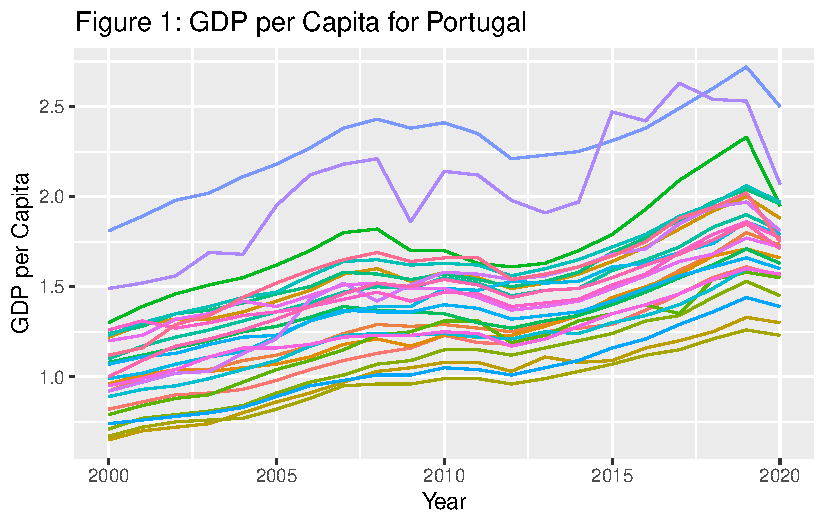
\includegraphics{MSB104_GR_1_Final_Assignment_research_article_files/figure-pdf/unnamed-chunk-7-1.pdf}

\begin{verbatim}
        GDP_per_capita
mean         1.4185524
median       1.3900000
std_dev      0.3702905
minimum      0.6500000
maximum      2.7200000
\end{verbatim}

By looking at figure for Portugal, we can see that the GDP per capita in
Portugal's regions appears to be fairly consistent. There is however
some regional variability. We can see signs of urbanisazation where the
regions around the big cities like Lisbon have a higher GDP per capita
compared to some more rural areas. Since Lisbon is the capital of
Portugal, there is probably a higher concentration of industries, making
it a economic center (which again makes the GDP per capita higher).

To continue, we can see that the mean is a little higher that the
median, something that might indicate that regions like Lisbon are
pulling up the average. If we compare the standard derivation for
Portugal with the other countries, we'll see that is fairly low in
comparison. This might mean that there is not a lot of variability
between the GDP per capita across different regions in Portugal. The gap
between minimum and maximum is also low compared to other countries,
something that'll also show us that the economic disparity in Portugal
might not be as high as it is in other countries.

\hypertarget{gdp-per-capita-france}{%
\subsubsection{GDP per capita France}\label{gdp-per-capita-france}}

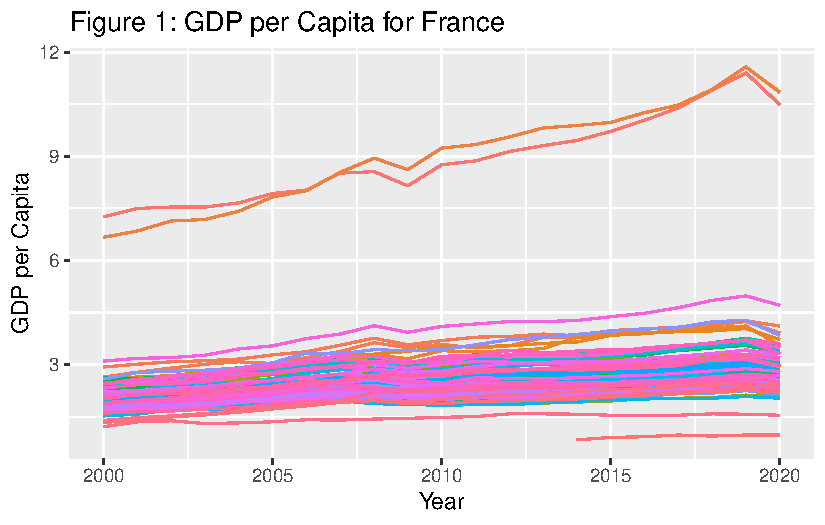
\includegraphics{MSB104_GR_1_Final_Assignment_research_article_files/figure-pdf/unnamed-chunk-10-1.pdf}

\begin{verbatim}
        GDP_per_capita
mean          2.630444
median        2.440000
std_dev       1.053767
minimum       0.830000
maximum      11.580000
\end{verbatim}

When looking at the figure for France, we see some regions have a much
higher GDP per capita compared to the other regions. The regions with
the highest GDP per capita for all years is the île-de-France region,
one that also includes Paris. This significant difference between the
regions with the highest GDP per capita and the lowest, shows us that
there is a high concentration of economic activity and wealth in a few
urban regions. Similar to Portugal, we see differences between urban and
rural regions.

Just as in Portugal, there is also a higher mean in France as well. On
the contary the data in France has higher standard derivation, and the
difference between minimum and maximum is larger. This strengthens
earlier figures showing, some regions having a high concentration of
wealth.

\hypertarget{gdp-per-capita-hungary}{%
\subsubsection{GDP per capita Hungary}\label{gdp-per-capita-hungary}}

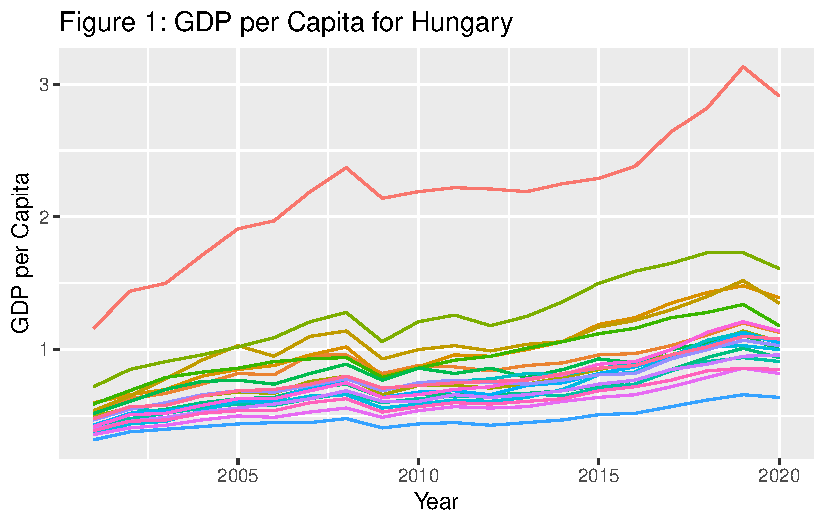
\includegraphics{MSB104_GR_1_Final_Assignment_research_article_files/figure-pdf/unnamed-chunk-13-1.pdf}

\begin{verbatim}
        GDP_per_capita
mean         0.8598000
median       0.7650000
std_dev      0.4059723
minimum      0.3200000
maximum      3.1300000
\end{verbatim}

In Hungary, most of the regions have similar GDP per Capita. One region
that sticks out by having a higher value, is the region of Budapest, the
capital.

This case also record the mean as higher vale than the median, high
standard derivation, and a large gap between minimum and maximum.

\hypertarget{gdp-per-capita-slovakia}{%
\subsubsection{GDP per capita Slovakia}\label{gdp-per-capita-slovakia}}

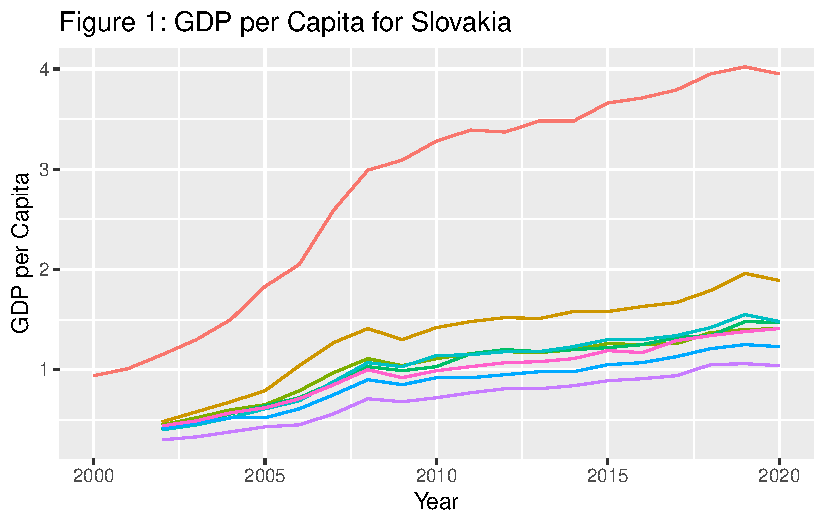
\includegraphics{MSB104_GR_1_Final_Assignment_research_article_files/figure-pdf/unnamed-chunk-16-1.pdf}

\begin{verbatim}
        GDP_per_capita
mean         1.2501948
median       1.0950000
std_dev      0.8018259
minimum      0.3000000
maximum      4.0200000
\end{verbatim}

Additionally, Slovakia, also have one region with much higher GDP per
capita than the rest of the regions. This region is Bratislava, which is
the biggest city and the capital, something that might point to this
city being the economic centre of Slovakia as well.

Slovakia follows the trend with higher mean than the median, and a large
gap between minimum and maximum. In addition, the standard derivation is
significantly high, meaning that there is some regions (or one region in
this case) that is further away from the rest of the regions in terms of
economic development.

\hypertarget{gdp-per-capita-denmark}{%
\subsubsection{GDP per capita Denmark}\label{gdp-per-capita-denmark}}

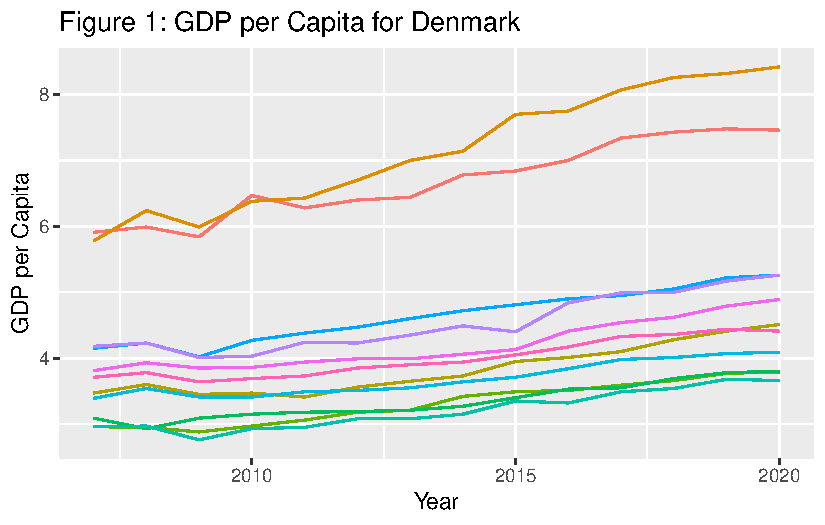
\includegraphics{MSB104_GR_1_Final_Assignment_research_article_files/figure-pdf/unnamed-chunk-19-1.pdf}

\begin{verbatim}
        GDP_per_capita
mean          4.419221
median        4.000000
std_dev       1.343933
minimum       2.760000
maximum       8.420000
\end{verbatim}

Lastly, we see similar pattern in Denmark, with the capital Copenhagen
being one of the regions with the highest GDP per capita.

Whith mean higher than the median, showing that regions like Copenhagen
possible dragging the mean up by population volume.

\hypertarget{part-1b-regional-inequity}{%
\subsection{Part 1B: Regional
Inequity}\label{part-1b-regional-inequity}}

\hypertarget{gini-coefficient-calculation}{%
\subsubsection{Gini Coefficient
Calculation}\label{gini-coefficient-calculation}}

In this part we will compute the population-weighted GDP Gini
coefficient for each European NUTS2 region in our assigned countries.

The gini coefficient can help us measure inequality in a distribution,
as is therefore a useful tool for us to use when we look at regional
inequity. The closer the gini coefficient is to 1, the bigger the
inequality is; a number closer to 0 equals equality. When looking at the
gini coefficient for NUTS 2 regions, we also get a better overview over
differences in income between different regions, and it also makes it
easier to find the reasons as to why there is a difference between the
regions Hasell \& Roser (2023).

With the use of the NUTS3 GDP per capita data and this formula:

\(GINW_j=\frac{1}{2 \bar{y_j}} \sum_{i}^{n_j}\sum_{l}^{n_j}\frac{p_i}{P_j} \frac{p_l}{P_j} |y_i-y_l|\)

After calculating the gini coefficients, we can see that there are some
similarities to the data we got from GDP per capita for NUTS 3 regions.
In order to see these similarities better, as well as look for other
important aspects that can be provided trough the calculations, we will
visualize the data in three different ways.

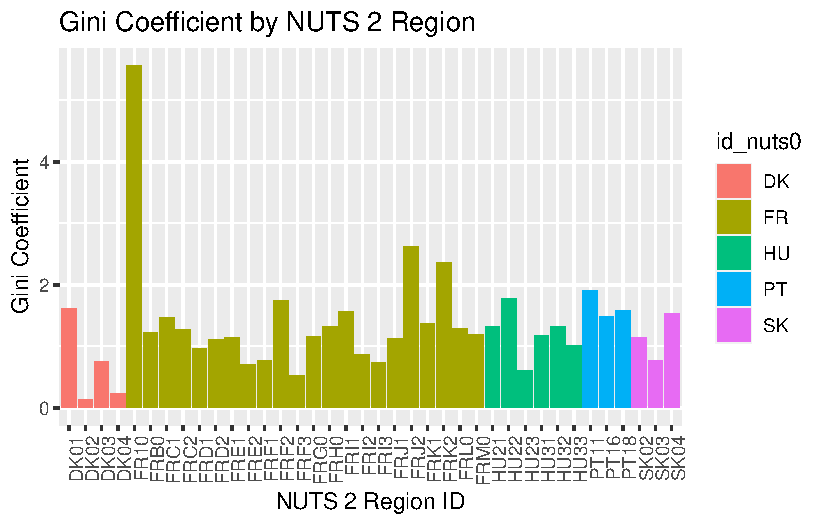
\includegraphics{MSB104_GR_1_Final_Assignment_research_article_files/figure-pdf/unnamed-chunk-23-1.pdf}

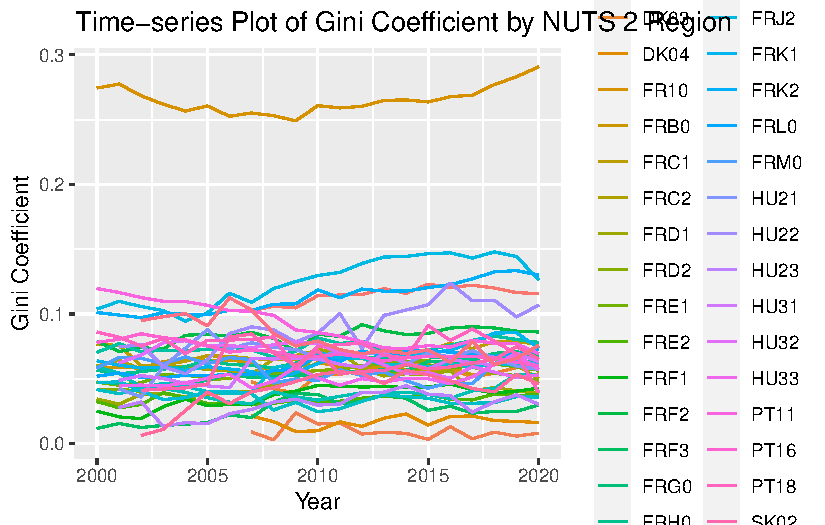
\includegraphics{MSB104_GR_1_Final_Assignment_research_article_files/figure-pdf/unnamed-chunk-24-1.pdf}

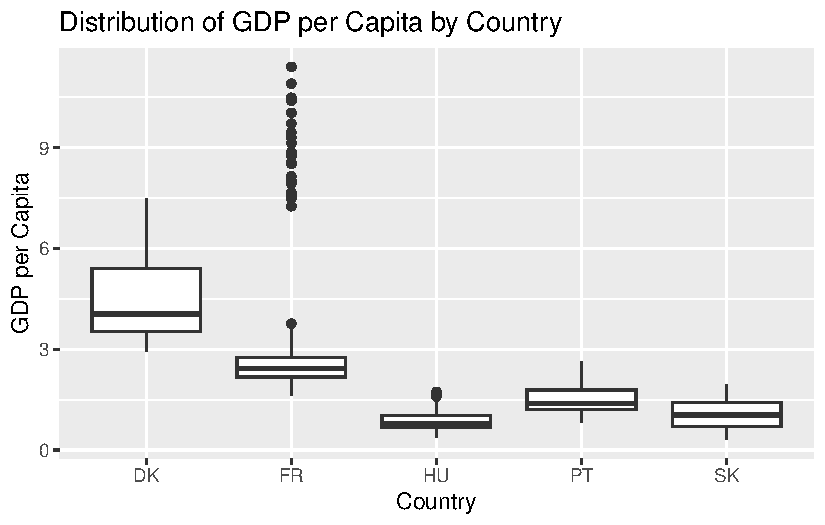
\includegraphics{MSB104_GR_1_Final_Assignment_research_article_files/figure-pdf/unnamed-chunk-25-1.pdf}

\hypertarget{cross-sectional-estimates}{%
\section{Cross sectional estimates}\label{cross-sectional-estimates}}

\hypertarget{part-2a-growth-and-inequity}{%
\subsection{Part 2A: Growth and
Inequity}\label{part-2a-growth-and-inequity}}

\hypertarget{data-acquisition}{%
\subsubsection{\texorpdfstring{\textbf{Data
acquisition}}{Data acquisition}}\label{data-acquisition}}

Firstly, the data is summerised for the year 2010 at the NUTS2 regional
level, focusing on economic metrics. Processing the dataset containing
the NUTS3 level. Thereafter, computing the total GDP and total
population for each NUTS2 region and year. Then, derive the GDP per
capita at the NUTS2 level by dividing the total GDP by the total
population again. Furthermore, narrowing down the dataset to
observations from the year 2010 where the Gini coefficient is positive.
Then adding, logarithmic transformations to linearize relationships or
to reduce the impact of extreme values.

The next step is making a data frame of NUTS2 2010 and grouping by NUTS0
country level variables, as well as allocating NUTS2 to selected
countries. Lastly presenting data in \textbf{table XXX} showing a count
of NUTS2 regions within each top-level region or country in the 2010
data.

The next step is, estimating a Linear Regression for All Countries using
cross sectional data from 2010, NUTS2.

\hypertarget{cross-sectional-analysis-1}{%
\subsubsection{\texorpdfstring{\textbf{Cross Sectional
Analysis}}{Cross Sectional Analysis}}\label{cross-sectional-analysis-1}}

With cross-sectional data analysis we create a snapshot of the year
2010. Cross-sectional data is simpler to manage and interpret than
time-series or panel data. With data from only one time point, we avoid
complications arising from temporal dynamics. Cross-sectional data
allows for the comparison of different regions at the same time, which
can be crucial for identifying disparities or differences between the
regions (Wooldridge, 2020).

\hypertarget{simple-linear-regression-model}{%
\subsubsection{\texorpdfstring{\textbf{Simple linear regression
model}}{Simple linear regression model}}\label{simple-linear-regression-model}}

In this part of the paper, we will carry out a simple regression model
and explore the effect of regional economic development, represented by
𝑦𝑗 (GDP per capita), on regional inequality, represented by 𝐺𝐼𝑁 𝐼𝑊𝑗. We
will do this to gain an understanding of the connection between economic
growth indicators such as GDP per capita and inequality might have. We
will explore if higher GDP per capita may lead to less or greater
inequality, and gain an understanding to what extent these variables are
related.

Unlike the traditional Gini coefficient, which treats all individuals
equally regardless of the population size of the region they reside in,
the weighted Gini considers the population size of each region,
assigning more weight to regions with larger populations.

In the context of regional inequality, this is particularly important
because it ensures that the income disparities in more populous regions
have a proportionally larger impact on the overall measure of
inequality. For instance, if a country has one region with a very high
level of income per capita but a small population, and another region
with a lower level of income per capita but a large population, the
weighted Gini coefficient would reflect the inequality experienced by a
larger portion of the country's population, providing a more accurate
picture of the national income distribution.

We use simple linear regression to model the relationship with the GINI
as the dependent variable and the natural logarithm of GDP per capita as
the independent variable. Capturing the relationship between regional
development and regional inequality for all regions in 2010.

\textbf{Model assumptions}

``The relationship between our dependent and independent variables is
linear, ensuring a clear and direct connection between them. Each
observation operates independently of the others, emphasizing the unique
contribution of every data point. Additionally, we expect
homoscedasticity, implying that the variance of the residuals remains
consistent regardless of the independent variable's level. It's also
crucial that, for any specified value of X, Y maintains a normal
distribution. And although more pertinent to multiple regression, it's
worth noting the absence of multicollinearity, ensuring that no two
predictors are closely correlated.''

\textbf{Model specification}

\[
Y_i = β_1 + β_2X_i + ε_i
\]

\(Y_i\) represent the dependent/ explained variable

\(X_i\) represent the independent/ explanatory variable

\(β_1\) represent the intercept/ constant

\(β_2\) represent the slope coefficient

\(ε_i\) represents the residuals or error in the prediction.

\textbf{Intercept (}β0\hspace{0pt}): represents the value of Y when X is
0.

\textbf{Slope (}β1\hspace{0pt}): Indicates the change in Y for a
one-unit change in X.

For our model we have:

\(GINI = \beta_{0} + \beta_{1} \cdot \text{GDP per capita} + \epsilon\)

\hypertarget{goodness-of-fit}{%
\paragraph{\texorpdfstring{\textbf{Goodness of
fit}}{Goodness of fit}}\label{goodness-of-fit}}

The goodness of fit in a simple linear regression model measures how
well the regression line approximates the real data points. The
regression line that best represents the data according to the least
squares criterion, which minimizes the sum of the squared vertical
distances of the points from the line.

R\^{}2 is a statistical measure that represents the proportion of the
variance for the dependent variable that's explained by the independent
variable. It ranges from 0 to 1. A higher R\^{}2 value indicates a
better fit of the model to the data.

R\^{}2 = 0 The model does not explain any of the variability of the
response data around its mean.

R\^{}2 = 1 The model explains all the variability of the response data
around its mean.

If the assumptions for a simple linear regression are met, it indicates
a good fit for the model. \ul{Plotting the data can provide a visual
indication of the goodness of fit.} The points should fall around a
straight line without clear patterns in the residuals. As it is crucial
to verify these assumptions before proceeding with interpreting the
results of the regression analysis.

\textbf{Residuals vs.~Fitted Values Plot} to check for homoscedasticity
and linearity. Ideally, this plot shows no pattern; the residuals are
randomly scattered around the horizontal line at zero. If there's a
pattern (like a curve or systematic spread of residuals), it suggests
non-linearity or heteroscedasticity.

\textbf{Normal Q-Q Plot} to check if the residuals are approximately
normally distributed. The points should fall roughly along a straight
line. Deviations from a straight line suggest deviations from normality.

 
  \providecommand{\huxb}[2]{\arrayrulecolor[RGB]{#1}\global\arrayrulewidth=#2pt}
  \providecommand{\huxvb}[2]{\color[RGB]{#1}\vrule width #2pt}
  \providecommand{\huxtpad}[1]{\rule{0pt}{#1}}
  \providecommand{\huxbpad}[1]{\rule[-#1]{0pt}{#1}}

\begin{table}[ht]
\begin{centerbox}
\begin{threeparttable}
 
\setlength{\tabcolsep}{0pt}
\begin{tabular}{l l}


\hhline{>{\huxb{0, 0, 0}{0.8}}->{\huxb{0, 0, 0}{0.8}}-}
\arrayrulecolor{black}

\multicolumn{1}{!{\huxvb{0, 0, 0}{0}}c!{\huxvb{0, 0, 0}{0}}}{\huxtpad{6pt + 1em}\centering \hspace{6pt}  \hspace{6pt}\huxbpad{6pt}} &
\multicolumn{1}{c!{\huxvb{0, 0, 0}{0}}}{\huxtpad{6pt + 1em}\centering \hspace{6pt} All \hspace{6pt}\huxbpad{6pt}} \tabularnewline[-0.5pt]


\hhline{>{\huxb{255, 255, 255}{0.4}}->{\huxb{0, 0, 0}{0.4}}-}
\arrayrulecolor{black}

\multicolumn{1}{!{\huxvb{0, 0, 0}{0}}l!{\huxvb{0, 0, 0}{0}}}{\huxtpad{6pt + 1em}\raggedright \hspace{6pt} (Intercept) \hspace{6pt}\huxbpad{6pt}} &
\multicolumn{1}{r!{\huxvb{0, 0, 0}{0}}}{\huxtpad{6pt + 1em}\raggedleft \hspace{6pt} 0.055 *** \hspace{6pt}\huxbpad{6pt}} \tabularnewline[-0.5pt]


\hhline{}
\arrayrulecolor{black}

\multicolumn{1}{!{\huxvb{0, 0, 0}{0}}l!{\huxvb{0, 0, 0}{0}}}{\huxtpad{6pt + 1em}\raggedright \hspace{6pt}  \hspace{6pt}\huxbpad{6pt}} &
\multicolumn{1}{r!{\huxvb{0, 0, 0}{0}}}{\huxtpad{6pt + 1em}\raggedleft \hspace{6pt} (0.010)\hphantom{0}\hphantom{0}\hphantom{0} \hspace{6pt}\huxbpad{6pt}} \tabularnewline[-0.5pt]


\hhline{}
\arrayrulecolor{black}

\multicolumn{1}{!{\huxvb{0, 0, 0}{0}}l!{\huxvb{0, 0, 0}{0}}}{\huxtpad{6pt + 1em}\raggedright \hspace{6pt} log\_GDP\_per\_capita \hspace{6pt}\huxbpad{6pt}} &
\multicolumn{1}{r!{\huxvb{0, 0, 0}{0}}}{\huxtpad{6pt + 1em}\raggedleft \hspace{6pt} 0.019\hphantom{0}\hphantom{0}\hphantom{0}\hphantom{0} \hspace{6pt}\huxbpad{6pt}} \tabularnewline[-0.5pt]


\hhline{}
\arrayrulecolor{black}

\multicolumn{1}{!{\huxvb{0, 0, 0}{0}}l!{\huxvb{0, 0, 0}{0}}}{\huxtpad{6pt + 1em}\raggedright \hspace{6pt}  \hspace{6pt}\huxbpad{6pt}} &
\multicolumn{1}{r!{\huxvb{0, 0, 0}{0}}}{\huxtpad{6pt + 1em}\raggedleft \hspace{6pt} (0.011)\hphantom{0}\hphantom{0}\hphantom{0} \hspace{6pt}\huxbpad{6pt}} \tabularnewline[-0.5pt]


\hhline{>{\huxb{255, 255, 255}{0.4}}->{\huxb{0, 0, 0}{0.4}}-}
\arrayrulecolor{black}

\multicolumn{1}{!{\huxvb{0, 0, 0}{0}}l!{\huxvb{0, 0, 0}{0}}}{\huxtpad{6pt + 1em}\raggedright \hspace{6pt} r.squared \hspace{6pt}\huxbpad{6pt}} &
\multicolumn{1}{r!{\huxvb{0, 0, 0}{0}}}{\huxtpad{6pt + 1em}\raggedleft \hspace{6pt} 0.080\hphantom{0}\hphantom{0}\hphantom{0}\hphantom{0} \hspace{6pt}\huxbpad{6pt}} \tabularnewline[-0.5pt]


\hhline{}
\arrayrulecolor{black}

\multicolumn{1}{!{\huxvb{0, 0, 0}{0}}l!{\huxvb{0, 0, 0}{0}}}{\huxtpad{6pt + 1em}\raggedright \hspace{6pt} adj.r.squared \hspace{6pt}\huxbpad{6pt}} &
\multicolumn{1}{r!{\huxvb{0, 0, 0}{0}}}{\huxtpad{6pt + 1em}\raggedleft \hspace{6pt} 0.055\hphantom{0}\hphantom{0}\hphantom{0}\hphantom{0} \hspace{6pt}\huxbpad{6pt}} \tabularnewline[-0.5pt]


\hhline{}
\arrayrulecolor{black}

\multicolumn{1}{!{\huxvb{0, 0, 0}{0}}l!{\huxvb{0, 0, 0}{0}}}{\huxtpad{6pt + 1em}\raggedright \hspace{6pt} statistic \hspace{6pt}\huxbpad{6pt}} &
\multicolumn{1}{r!{\huxvb{0, 0, 0}{0}}}{\huxtpad{6pt + 1em}\raggedleft \hspace{6pt} 3.142\hphantom{0}\hphantom{0}\hphantom{0}\hphantom{0} \hspace{6pt}\huxbpad{6pt}} \tabularnewline[-0.5pt]


\hhline{}
\arrayrulecolor{black}

\multicolumn{1}{!{\huxvb{0, 0, 0}{0}}l!{\huxvb{0, 0, 0}{0}}}{\huxtpad{6pt + 1em}\raggedright \hspace{6pt} p.value \hspace{6pt}\huxbpad{6pt}} &
\multicolumn{1}{r!{\huxvb{0, 0, 0}{0}}}{\huxtpad{6pt + 1em}\raggedleft \hspace{6pt} 0.085\hphantom{0}\hphantom{0}\hphantom{0}\hphantom{0} \hspace{6pt}\huxbpad{6pt}} \tabularnewline[-0.5pt]


\hhline{>{\huxb{0, 0, 0}{0.8}}->{\huxb{0, 0, 0}{0.8}}-}
\arrayrulecolor{black}

\multicolumn{2}{!{\huxvb{0, 0, 0}{0}}l!{\huxvb{0, 0, 0}{0}}}{\huxtpad{6pt + 1em}\raggedright \hspace{6pt}  *** p $<$ 0.001;  ** p $<$ 0.01;  * p $<$ 0.05. \hspace{6pt}\huxbpad{6pt}} \tabularnewline[-0.5pt]


\hhline{}
\arrayrulecolor{black}
\end{tabular}
\end{threeparttable}\par\end{centerbox}

\end{table}
 

Regression statistics of all countries for the year 2010

 
  \providecommand{\huxb}[2]{\arrayrulecolor[RGB]{#1}\global\arrayrulewidth=#2pt}
  \providecommand{\huxvb}[2]{\color[RGB]{#1}\vrule width #2pt}
  \providecommand{\huxtpad}[1]{\rule{0pt}{#1}}
  \providecommand{\huxbpad}[1]{\rule[-#1]{0pt}{#1}}

\begin{table}[ht]
\begin{centerbox}
\begin{threeparttable}
 
\setlength{\tabcolsep}{0pt}
\begin{tabular}{l l l l l l}


\hhline{>{\huxb{0, 0, 0}{0.8}}->{\huxb{0, 0, 0}{0.8}}->{\huxb{0, 0, 0}{0.8}}->{\huxb{0, 0, 0}{0.8}}->{\huxb{0, 0, 0}{0.8}}->{\huxb{0, 0, 0}{0.8}}-}
\arrayrulecolor{black}

\multicolumn{1}{!{\huxvb{0, 0, 0}{0}}c!{\huxvb{0, 0, 0}{0}}}{\huxtpad{6pt + 1em}\centering \hspace{6pt}  \hspace{6pt}\huxbpad{6pt}} &
\multicolumn{1}{c!{\huxvb{0, 0, 0}{0}}}{\huxtpad{6pt + 1em}\centering \hspace{6pt} SK \hspace{6pt}\huxbpad{6pt}} &
\multicolumn{1}{c!{\huxvb{0, 0, 0}{0}}}{\huxtpad{6pt + 1em}\centering \hspace{6pt} DK \hspace{6pt}\huxbpad{6pt}} &
\multicolumn{1}{c!{\huxvb{0, 0, 0}{0}}}{\huxtpad{6pt + 1em}\centering \hspace{6pt} HU \hspace{6pt}\huxbpad{6pt}} &
\multicolumn{1}{c!{\huxvb{0, 0, 0}{0}}}{\huxtpad{6pt + 1em}\centering \hspace{6pt} PT \hspace{6pt}\huxbpad{6pt}} &
\multicolumn{1}{c!{\huxvb{0, 0, 0}{0}}}{\huxtpad{6pt + 1em}\centering \hspace{6pt} FR \hspace{6pt}\huxbpad{6pt}} \tabularnewline[-0.5pt]


\hhline{>{\huxb{255, 255, 255}{0.4}}->{\huxb{0, 0, 0}{0.4}}->{\huxb{0, 0, 0}{0.4}}->{\huxb{0, 0, 0}{0.4}}->{\huxb{0, 0, 0}{0.4}}->{\huxb{0, 0, 0}{0.4}}-}
\arrayrulecolor{black}

\multicolumn{1}{!{\huxvb{0, 0, 0}{0}}l!{\huxvb{0, 0, 0}{0}}}{\huxtpad{6pt + 1em}\raggedright \hspace{6pt} (Intercept) \hspace{6pt}\huxbpad{6pt}} &
\multicolumn{1}{r!{\huxvb{0, 0, 0}{0}}}{\huxtpad{6pt + 1em}\raggedleft \hspace{6pt} 0.069\hphantom{0} \hspace{6pt}\huxbpad{6pt}} &
\multicolumn{1}{r!{\huxvb{0, 0, 0}{0}}}{\huxtpad{6pt + 1em}\raggedleft \hspace{6pt} -0.127\hphantom{0} \hspace{6pt}\huxbpad{6pt}} &
\multicolumn{1}{r!{\huxvb{0, 0, 0}{0}}}{\huxtpad{6pt + 1em}\raggedleft \hspace{6pt} 0.075 ** \hspace{6pt}\huxbpad{6pt}} &
\multicolumn{1}{r!{\huxvb{0, 0, 0}{0}}}{\huxtpad{6pt + 1em}\raggedleft \hspace{6pt} 0.079\hphantom{0} \hspace{6pt}\huxbpad{6pt}} &
\multicolumn{1}{r!{\huxvb{0, 0, 0}{0}}}{\huxtpad{6pt + 1em}\raggedleft \hspace{6pt} -0.028\hphantom{0}\hphantom{0}\hphantom{0}\hphantom{0} \hspace{6pt}\huxbpad{6pt}} \tabularnewline[-0.5pt]


\hhline{}
\arrayrulecolor{black}

\multicolumn{1}{!{\huxvb{0, 0, 0}{0}}l!{\huxvb{0, 0, 0}{0}}}{\huxtpad{6pt + 1em}\raggedright \hspace{6pt}  \hspace{6pt}\huxbpad{6pt}} &
\multicolumn{1}{r!{\huxvb{0, 0, 0}{0}}}{\huxtpad{6pt + 1em}\raggedleft \hspace{6pt} (0.010) \hspace{6pt}\huxbpad{6pt}} &
\multicolumn{1}{r!{\huxvb{0, 0, 0}{0}}}{\huxtpad{6pt + 1em}\raggedleft \hspace{6pt} (0.085) \hspace{6pt}\huxbpad{6pt}} &
\multicolumn{1}{r!{\huxvb{0, 0, 0}{0}}}{\huxtpad{6pt + 1em}\raggedleft \hspace{6pt} (0.010)\hphantom{0}\hphantom{0} \hspace{6pt}\huxbpad{6pt}} &
\multicolumn{1}{r!{\huxvb{0, 0, 0}{0}}}{\huxtpad{6pt + 1em}\raggedleft \hspace{6pt} (0.015) \hspace{6pt}\huxbpad{6pt}} &
\multicolumn{1}{r!{\huxvb{0, 0, 0}{0}}}{\huxtpad{6pt + 1em}\raggedleft \hspace{6pt} (0.026)\hphantom{0}\hphantom{0}\hphantom{0} \hspace{6pt}\huxbpad{6pt}} \tabularnewline[-0.5pt]


\hhline{}
\arrayrulecolor{black}

\multicolumn{1}{!{\huxvb{0, 0, 0}{0}}l!{\huxvb{0, 0, 0}{0}}}{\huxtpad{6pt + 1em}\raggedright \hspace{6pt} log\_GDP\_per\_capita \hspace{6pt}\huxbpad{6pt}} &
\multicolumn{1}{r!{\huxvb{0, 0, 0}{0}}}{\huxtpad{6pt + 1em}\raggedleft \hspace{6pt} -0.018\hphantom{0} \hspace{6pt}\huxbpad{6pt}} &
\multicolumn{1}{r!{\huxvb{0, 0, 0}{0}}}{\huxtpad{6pt + 1em}\raggedleft \hspace{6pt} 0.124\hphantom{0} \hspace{6pt}\huxbpad{6pt}} &
\multicolumn{1}{r!{\huxvb{0, 0, 0}{0}}}{\huxtpad{6pt + 1em}\raggedleft \hspace{6pt} 0.049\hphantom{0}\hphantom{0}\hphantom{0} \hspace{6pt}\huxbpad{6pt}} &
\multicolumn{1}{r!{\huxvb{0, 0, 0}{0}}}{\huxtpad{6pt + 1em}\raggedleft \hspace{6pt} -0.008\hphantom{0} \hspace{6pt}\huxbpad{6pt}} &
\multicolumn{1}{r!{\huxvb{0, 0, 0}{0}}}{\huxtpad{6pt + 1em}\raggedleft \hspace{6pt} 0.107 *** \hspace{6pt}\huxbpad{6pt}} \tabularnewline[-0.5pt]


\hhline{}
\arrayrulecolor{black}

\multicolumn{1}{!{\huxvb{0, 0, 0}{0}}l!{\huxvb{0, 0, 0}{0}}}{\huxtpad{6pt + 1em}\raggedright \hspace{6pt}  \hspace{6pt}\huxbpad{6pt}} &
\multicolumn{1}{r!{\huxvb{0, 0, 0}{0}}}{\huxtpad{6pt + 1em}\raggedleft \hspace{6pt} (0.034) \hspace{6pt}\huxbpad{6pt}} &
\multicolumn{1}{r!{\huxvb{0, 0, 0}{0}}}{\huxtpad{6pt + 1em}\raggedleft \hspace{6pt} (0.059) \hspace{6pt}\huxbpad{6pt}} &
\multicolumn{1}{r!{\huxvb{0, 0, 0}{0}}}{\huxtpad{6pt + 1em}\raggedleft \hspace{6pt} (0.029)\hphantom{0}\hphantom{0} \hspace{6pt}\huxbpad{6pt}} &
\multicolumn{1}{r!{\huxvb{0, 0, 0}{0}}}{\huxtpad{6pt + 1em}\raggedleft \hspace{6pt} (0.030) \hspace{6pt}\huxbpad{6pt}} &
\multicolumn{1}{r!{\huxvb{0, 0, 0}{0}}}{\huxtpad{6pt + 1em}\raggedleft \hspace{6pt} (0.026)\hphantom{0}\hphantom{0}\hphantom{0} \hspace{6pt}\huxbpad{6pt}} \tabularnewline[-0.5pt]


\hhline{>{\huxb{255, 255, 255}{0.4}}->{\huxb{0, 0, 0}{0.4}}->{\huxb{0, 0, 0}{0.4}}->{\huxb{0, 0, 0}{0.4}}->{\huxb{0, 0, 0}{0.4}}->{\huxb{0, 0, 0}{0.4}}-}
\arrayrulecolor{black}

\multicolumn{1}{!{\huxvb{0, 0, 0}{0}}l!{\huxvb{0, 0, 0}{0}}}{\huxtpad{6pt + 1em}\raggedright \hspace{6pt} r.squared \hspace{6pt}\huxbpad{6pt}} &
\multicolumn{1}{r!{\huxvb{0, 0, 0}{0}}}{\huxtpad{6pt + 1em}\raggedleft \hspace{6pt} 0.221\hphantom{0} \hspace{6pt}\huxbpad{6pt}} &
\multicolumn{1}{r!{\huxvb{0, 0, 0}{0}}}{\huxtpad{6pt + 1em}\raggedleft \hspace{6pt} 0.689\hphantom{0} \hspace{6pt}\huxbpad{6pt}} &
\multicolumn{1}{r!{\huxvb{0, 0, 0}{0}}}{\huxtpad{6pt + 1em}\raggedleft \hspace{6pt} 0.410\hphantom{0}\hphantom{0}\hphantom{0} \hspace{6pt}\huxbpad{6pt}} &
\multicolumn{1}{r!{\huxvb{0, 0, 0}{0}}}{\huxtpad{6pt + 1em}\raggedleft \hspace{6pt} 0.067\hphantom{0} \hspace{6pt}\huxbpad{6pt}} &
\multicolumn{1}{r!{\huxvb{0, 0, 0}{0}}}{\huxtpad{6pt + 1em}\raggedleft \hspace{6pt} 0.457\hphantom{0}\hphantom{0}\hphantom{0}\hphantom{0} \hspace{6pt}\huxbpad{6pt}} \tabularnewline[-0.5pt]


\hhline{}
\arrayrulecolor{black}

\multicolumn{1}{!{\huxvb{0, 0, 0}{0}}l!{\huxvb{0, 0, 0}{0}}}{\huxtpad{6pt + 1em}\raggedright \hspace{6pt} adj.r.squared \hspace{6pt}\huxbpad{6pt}} &
\multicolumn{1}{r!{\huxvb{0, 0, 0}{0}}}{\huxtpad{6pt + 1em}\raggedleft \hspace{6pt} -0.558\hphantom{0} \hspace{6pt}\huxbpad{6pt}} &
\multicolumn{1}{r!{\huxvb{0, 0, 0}{0}}}{\huxtpad{6pt + 1em}\raggedleft \hspace{6pt} 0.534\hphantom{0} \hspace{6pt}\huxbpad{6pt}} &
\multicolumn{1}{r!{\huxvb{0, 0, 0}{0}}}{\huxtpad{6pt + 1em}\raggedleft \hspace{6pt} 0.262\hphantom{0}\hphantom{0}\hphantom{0} \hspace{6pt}\huxbpad{6pt}} &
\multicolumn{1}{r!{\huxvb{0, 0, 0}{0}}}{\huxtpad{6pt + 1em}\raggedleft \hspace{6pt} -0.866\hphantom{0} \hspace{6pt}\huxbpad{6pt}} &
\multicolumn{1}{r!{\huxvb{0, 0, 0}{0}}}{\huxtpad{6pt + 1em}\raggedleft \hspace{6pt} 0.430\hphantom{0}\hphantom{0}\hphantom{0}\hphantom{0} \hspace{6pt}\huxbpad{6pt}} \tabularnewline[-0.5pt]


\hhline{}
\arrayrulecolor{black}

\multicolumn{1}{!{\huxvb{0, 0, 0}{0}}l!{\huxvb{0, 0, 0}{0}}}{\huxtpad{6pt + 1em}\raggedright \hspace{6pt} statistic \hspace{6pt}\huxbpad{6pt}} &
\multicolumn{1}{r!{\huxvb{0, 0, 0}{0}}}{\huxtpad{6pt + 1em}\raggedleft \hspace{6pt} 0.284\hphantom{0} \hspace{6pt}\huxbpad{6pt}} &
\multicolumn{1}{r!{\huxvb{0, 0, 0}{0}}}{\huxtpad{6pt + 1em}\raggedleft \hspace{6pt} 4.432\hphantom{0} \hspace{6pt}\huxbpad{6pt}} &
\multicolumn{1}{r!{\huxvb{0, 0, 0}{0}}}{\huxtpad{6pt + 1em}\raggedleft \hspace{6pt} 2.778\hphantom{0}\hphantom{0}\hphantom{0} \hspace{6pt}\huxbpad{6pt}} &
\multicolumn{1}{r!{\huxvb{0, 0, 0}{0}}}{\huxtpad{6pt + 1em}\raggedleft \hspace{6pt} 0.072\hphantom{0} \hspace{6pt}\huxbpad{6pt}} &
\multicolumn{1}{r!{\huxvb{0, 0, 0}{0}}}{\huxtpad{6pt + 1em}\raggedleft \hspace{6pt} 16.820\hphantom{0}\hphantom{0}\hphantom{0}\hphantom{0} \hspace{6pt}\huxbpad{6pt}} \tabularnewline[-0.5pt]


\hhline{}
\arrayrulecolor{black}

\multicolumn{1}{!{\huxvb{0, 0, 0}{0}}l!{\huxvb{0, 0, 0}{0}}}{\huxtpad{6pt + 1em}\raggedright \hspace{6pt} p.value \hspace{6pt}\huxbpad{6pt}} &
\multicolumn{1}{r!{\huxvb{0, 0, 0}{0}}}{\huxtpad{6pt + 1em}\raggedleft \hspace{6pt} 0.689\hphantom{0} \hspace{6pt}\huxbpad{6pt}} &
\multicolumn{1}{r!{\huxvb{0, 0, 0}{0}}}{\huxtpad{6pt + 1em}\raggedleft \hspace{6pt} 0.170\hphantom{0} \hspace{6pt}\huxbpad{6pt}} &
\multicolumn{1}{r!{\huxvb{0, 0, 0}{0}}}{\huxtpad{6pt + 1em}\raggedleft \hspace{6pt} 0.171\hphantom{0}\hphantom{0}\hphantom{0} \hspace{6pt}\huxbpad{6pt}} &
\multicolumn{1}{r!{\huxvb{0, 0, 0}{0}}}{\huxtpad{6pt + 1em}\raggedleft \hspace{6pt} 0.833\hphantom{0} \hspace{6pt}\huxbpad{6pt}} &
\multicolumn{1}{r!{\huxvb{0, 0, 0}{0}}}{\huxtpad{6pt + 1em}\raggedleft \hspace{6pt} 0.001\hphantom{0}\hphantom{0}\hphantom{0}\hphantom{0} \hspace{6pt}\huxbpad{6pt}} \tabularnewline[-0.5pt]


\hhline{>{\huxb{0, 0, 0}{0.8}}->{\huxb{0, 0, 0}{0.8}}->{\huxb{0, 0, 0}{0.8}}->{\huxb{0, 0, 0}{0.8}}->{\huxb{0, 0, 0}{0.8}}->{\huxb{0, 0, 0}{0.8}}-}
\arrayrulecolor{black}

\multicolumn{6}{!{\huxvb{0, 0, 0}{0}}l!{\huxvb{0, 0, 0}{0}}}{\huxtpad{6pt + 1em}\raggedright \hspace{6pt}  *** p $<$ 0.001;  ** p $<$ 0.01;  * p $<$ 0.05. \hspace{6pt}\huxbpad{6pt}} \tabularnewline[-0.5pt]


\hhline{}
\arrayrulecolor{black}
\end{tabular}
\end{threeparttable}\par\end{centerbox}

\end{table}
 

Regression statistics of all countries seperately for the year 2010

\textbf{Model Diagnostics}

We'll now look at some of the numbers we got from the linear regression
model (for all countries combined):

\begin{itemize}
\item
  Coefficients:

  \begin{itemize}
  \item
    Intercept is 0.0551 (expected value of gini when GDP per capita is
    0). Statistically significant (indicated by p-value).
  \item
    Estimated coefficient for GDP per capita is 0.0193, if the natural
    logarithm of GDP per capita increase by one, then the gini
    coefficient will increase by 0.0193. The p-value associated with the
    coefficent is however not statistically significant at 5\% level.
  \end{itemize}
\item
  Goodnes of fit:

  \begin{itemize}
  \item
    Multiple R-squared (0.08028) indicate that around 8\% of the
    variability in the GINI coefficient is explained by the model. This
    is low, which can suggest that the model dosen't explain the
    variation in gini.
  \item
    Adjusted R-squared is even lower (0.05474), is therefore expected
    that the model dosen't really explain the variance in the dependent
    variable (gini).
  \end{itemize}
\item
  Model significance:

  \begin{itemize}
  \tightlist
  \item
    The F-statistic (3.142) indicate the significance of the regression
    model. We can see here, that with the p-value of 0.08474, the model
    isn't significant at a 5\% level.
  \end{itemize}
\end{itemize}

By looking at these numbers, we can see that the model may not reliably
predict the gini coefficient. It also suggest that GDP per capita may
not be a valid predictor of the gini coefficient.

We also examined our selected countries seperately in order to see how
the reliability and validity of the model might vary between countries.
However, since there are too few observations for most of the countries,
it makes it hard to make a conclusion of the reliability. What we can
see from this examination, is that the models for Denmark, Portugal and
Slovakia are not statistically significant. France seem however to have
significant coefficiants, and Hungary have a moderate R-squared (but
lacks significance in the slope).

\textbf{Ordinary Least Squares (OLS) Estimation}

``The OLS method is employed to identify the best-fitting linear
relationship between the dependent and independent variables, aiming to
minimize the sum of squared residuals. This technique ensures that the
estimations of the intercept (β0) and slope (β1) yield the least
possible cumulative discrepancy between the actual and predicted values.
The strength of OLS lies in its closed-form solution, providing a
straightforward computation of coefficients directly from the data-set,
without necessitating iterative procedures.

Furthermore, when the classical linear regression assumptions are met,
OLS guarantees that the estimators are BLUE, ensuring their unbiasedness
and efficiency. This is particularly crucial in econometric analysis,
where the precision and reliability of parameter estimates are paramount
for policy implications and economic interpretations. The foundation
assumptions of linear regression, including linearity, independence,
homoscedasticity, and normality of residuals, are prerequisites for OLS
to attain these desirable properties. It is imperative, therefore, to
conduct diagnostic tests and assess the validity of these assumptions to
ensure the robustness of the OLS estimators used in our analysis.''

\hypertarget{assumptions}{%
\subsubsection{\texorpdfstring{\textbf{Assumptions}}{Assumptions}}\label{assumptions}}

\textbf{I. Linearity}

The relationship between the independent variable X and the dependent
variable Y is linear. This means that changes in X are associated with
proportional changes in Y. A straight line should provide a good fit to
the data points when plotted on a graph.

You can create a scatter plot of Y versus X and visually inspect whether
a straight line could well represent the relationship. Alternatively,
you can plot the residuals versus the fitted values and check for any
obvious patterns or non-linearity.

\textbf{II. Independence:}

Observations are independent of each other. The value of Y for one
observation should not depend on the value of Y for any other
observation.

This assumption is more about study design and data collection. Ensure
that your observations are not correlated in time or space. For example,
if you're analyzing economic data across regions, make sure that the
regions are not influencing each other.

\textbf{III. Homoscedasticity (Equal Variance):}

The variance of the residuals (the errors) is constant across all levels
of X. This means that the spread or ``width'' of the residuals should
remain roughly the same across all values of the independent variable.

A plot of residuals versus fitted values should show a random scatter
and not display any funnel-like shapes (wider at one end).

\textbf{IV. Normality of Residuals:}

The residuals (the differences between observed and predicted values)
are normally distributed. This assumption is particularly important for
hypothesis testing and creating confidence intervals.

A Quantile-Quantile (Q-Q) plot of the residuals can show if they follow
a normal distribution. The points should fall roughly along a straight
line.

\textbf{V. No Perfect Multicollinearity (Specific to Multiple
Regression)}

In multiple regression settings, this assumes that no independent
variable is a perfect linear function of any other independent
variables. While this is more pertinent to multiple linear regression,
it is crucial there because high correlation between independent
variables can lead to unstable coefficient estimates.

Checking the variance inflation factor (VIF) for each variable; a VIF
above 5-10 indicates a problematic amount of collinearity.

\textbf{Visualization}

\includegraphics{MSB104_GR_1_Final_Assignment_research_article_files/figure-pdf/unnamed-chunk-29-1.pdf}

\includegraphics{MSB104_GR_1_Final_Assignment_research_article_files/figure-pdf/unnamed-chunk-29-2.pdf}

We've made two plots that can help us understand the relationship
between GDP per capita and the Gini coefficient, and that together with
the regression statistics can help with discussing if the classical OLS
assumptions hold for the model. The first one is a plot that shows us
residuals vs fitted values, which can help us check the homoscedasticity
assumption of a linear regression model. The residuals should be
randomly scattered around the horisontal 0 line, something that can
inducate that the variances of the error terms are constant. In our
plot, the residuals are in some extent randomly distributed, and there
is also no clear pattern; this suggest that there is likely no
significant issues with heteroscedasticity or non-linearity.

The other plot - normal Q-Q plot - is used to assess if the residuals of
the linear model are normally distributed. In our plot, most of the
points follow the line closely, suggesting that the residuals are
normally distributed. There are however some outliers in the tails, that
suggest some variation from normality.

In both of these plots, we can see that there are some outliers, these
can affect the fit of the model. These outliers might come from regions
that have a high GDP per capita compared to rest of the regions, like
Paris in France that is a financial hub.

\begin{verbatim}
`geom_smooth()` using formula = 'y ~ x'
\end{verbatim}

\begin{figure}

{\centering \includegraphics{MSB104_GR_1_Final_Assignment_research_article_files/figure-pdf/fig_scatterplot-all-1.pdf}

}

\caption{Relationship Between GDP per Capita and Gini}

\end{figure}

In this plot we are visualizing the relationship between GDP per capita
and gini by using a mix of the two previous plots. We can here as well,
see extreme outliers.

\hypertarget{part-2b-exploring-other-determinants-of-inequity}{%
\subsection{Part 2B: Exploring Other Determinants of
Inequity}\label{part-2b-exploring-other-determinants-of-inequity}}

\hypertarget{i.-data-acquisition}{%
\subsubsection{I. Data Acquisition}\label{i.-data-acquisition}}

Se data section for more specifications on the added population nut2,
transport infrastructure and education.

In order to conduct a Multiple Linear Regression model, we need to have
some independent variables to use in the model and compare them with the
dependent variable. The first variable, education, can explain income
inequality, since it can influence income distribution in a region. If
access to education is unequal, then higher education levels might
incease income disparities (Rodriguez-Pose \& Tselios, 2008). The
population density, our second variable, can explain inequality since
regions with a higher population density might have different economic
behaviours. Our last variable, rail network (infrastructure), can
influence economic development and accessibility, which also can affect
income inequality in a region (Chatterjee \& Turnovsky, 2012).

\hypertarget{ii.-multiple-linear-regression-model}{%
\subsubsection{II. Multiple Linear Regression
Model}\label{ii.-multiple-linear-regression-model}}

Multiple Linear Regression (MLR) extends simple linear regression to
incorporate multiple explanatory variables, allowing us to examine how
multiple factors impact a dependent variable. Choosing a data set from
the year 2010 that consists of various regions, with data on each
region's economic indicators, demographic variables, and other factors.
Our aim is to understand how these variables collectively affect
regional inequality.

We will in this part do a Multiple Linear Regression model by using the
variables education (in percentage of pupils and students in education,
\% of total population), population density and rail network in km. This
model will tell us if these variables can help explain change in the
gini coefficient.

In both our simple linear regression model, and now in our multiple
linear regression model, we use the logarithmic function which makes it
easier to linearize the relationship between the variables. By using it
for GDP per capita, we can reflect changes more effectively. For rail
network and population density, the logarithm function ensure that the
model capture proportional changes and deals better with the wide range
of values.

 
  \providecommand{\huxb}[2]{\arrayrulecolor[RGB]{#1}\global\arrayrulewidth=#2pt}
  \providecommand{\huxvb}[2]{\color[RGB]{#1}\vrule width #2pt}
  \providecommand{\huxtpad}[1]{\rule{0pt}{#1}}
  \providecommand{\huxbpad}[1]{\rule[-#1]{0pt}{#1}}

\begin{table}[ht]
\begin{centerbox}
\begin{threeparttable}
 
\setlength{\tabcolsep}{0pt}
\begin{tabular}{l l l l}


\hhline{>{\huxb{0, 0, 0}{0.8}}->{\huxb{0, 0, 0}{0.8}}->{\huxb{0, 0, 0}{0.8}}->{\huxb{0, 0, 0}{0.8}}-}
\arrayrulecolor{black}

\multicolumn{1}{!{\huxvb{0, 0, 0}{0}}c!{\huxvb{0, 0, 0}{0}}}{\huxtpad{6pt + 1em}\centering \hspace{6pt}  \hspace{6pt}\huxbpad{6pt}} &
\multicolumn{1}{c!{\huxvb{0, 0, 0}{0}}}{\huxtpad{6pt + 1em}\centering \hspace{6pt} Model \hspace{6pt}\huxbpad{6pt}} &
\multicolumn{1}{c!{\huxvb{0, 0, 0}{0}}}{\huxtpad{6pt + 1em}\centering \hspace{6pt} Model 2 \hspace{6pt}\huxbpad{6pt}} &
\multicolumn{1}{c!{\huxvb{0, 0, 0}{0}}}{\huxtpad{6pt + 1em}\centering \hspace{6pt} Model 3 \hspace{6pt}\huxbpad{6pt}} \tabularnewline[-0.5pt]


\hhline{>{\huxb{255, 255, 255}{0.4}}->{\huxb{0, 0, 0}{0.4}}->{\huxb{0, 0, 0}{0.4}}->{\huxb{0, 0, 0}{0.4}}-}
\arrayrulecolor{black}

\multicolumn{1}{!{\huxvb{0, 0, 0}{0}}l!{\huxvb{0, 0, 0}{0}}}{\huxtpad{6pt + 1em}\raggedright \hspace{6pt} (Intercept) \hspace{6pt}\huxbpad{6pt}} &
\multicolumn{1}{r!{\huxvb{0, 0, 0}{0}}}{\huxtpad{6pt + 1em}\raggedleft \hspace{6pt} 0.050\hphantom{0} \hspace{6pt}\huxbpad{6pt}} &
\multicolumn{1}{r!{\huxvb{0, 0, 0}{0}}}{\huxtpad{6pt + 1em}\raggedleft \hspace{6pt} 0.008\hphantom{0}\hphantom{0}\hphantom{0} \hspace{6pt}\huxbpad{6pt}} &
\multicolumn{1}{r!{\huxvb{0, 0, 0}{0}}}{\huxtpad{6pt + 1em}\raggedleft \hspace{6pt} -0.206\hphantom{0}\hphantom{0} \hspace{6pt}\huxbpad{6pt}} \tabularnewline[-0.5pt]


\hhline{}
\arrayrulecolor{black}

\multicolumn{1}{!{\huxvb{0, 0, 0}{0}}l!{\huxvb{0, 0, 0}{0}}}{\huxtpad{6pt + 1em}\raggedright \hspace{6pt}  \hspace{6pt}\huxbpad{6pt}} &
\multicolumn{1}{r!{\huxvb{0, 0, 0}{0}}}{\huxtpad{6pt + 1em}\raggedleft \hspace{6pt} (0.091) \hspace{6pt}\huxbpad{6pt}} &
\multicolumn{1}{r!{\huxvb{0, 0, 0}{0}}}{\huxtpad{6pt + 1em}\raggedleft \hspace{6pt} (0.078)\hphantom{0}\hphantom{0} \hspace{6pt}\huxbpad{6pt}} &
\multicolumn{1}{r!{\huxvb{0, 0, 0}{0}}}{\huxtpad{6pt + 1em}\raggedleft \hspace{6pt} (0.114)\hphantom{0} \hspace{6pt}\huxbpad{6pt}} \tabularnewline[-0.5pt]


\hhline{}
\arrayrulecolor{black}

\multicolumn{1}{!{\huxvb{0, 0, 0}{0}}l!{\huxvb{0, 0, 0}{0}}}{\huxtpad{6pt + 1em}\raggedright \hspace{6pt} log\_GDP\_per\_capita \hspace{6pt}\huxbpad{6pt}} &
\multicolumn{1}{r!{\huxvb{0, 0, 0}{0}}}{\huxtpad{6pt + 1em}\raggedleft \hspace{6pt} 0.020\hphantom{0} \hspace{6pt}\huxbpad{6pt}} &
\multicolumn{1}{r!{\huxvb{0, 0, 0}{0}}}{\huxtpad{6pt + 1em}\raggedleft \hspace{6pt} 0.011\hphantom{0}\hphantom{0}\hphantom{0} \hspace{6pt}\huxbpad{6pt}} &
\multicolumn{1}{r!{\huxvb{0, 0, 0}{0}}}{\huxtpad{6pt + 1em}\raggedleft \hspace{6pt} 0.017\hphantom{0}\hphantom{0} \hspace{6pt}\huxbpad{6pt}} \tabularnewline[-0.5pt]


\hhline{}
\arrayrulecolor{black}

\multicolumn{1}{!{\huxvb{0, 0, 0}{0}}l!{\huxvb{0, 0, 0}{0}}}{\huxtpad{6pt + 1em}\raggedright \hspace{6pt}  \hspace{6pt}\huxbpad{6pt}} &
\multicolumn{1}{r!{\huxvb{0, 0, 0}{0}}}{\huxtpad{6pt + 1em}\raggedleft \hspace{6pt} (0.014) \hspace{6pt}\huxbpad{6pt}} &
\multicolumn{1}{r!{\huxvb{0, 0, 0}{0}}}{\huxtpad{6pt + 1em}\raggedleft \hspace{6pt} (0.012)\hphantom{0}\hphantom{0} \hspace{6pt}\huxbpad{6pt}} &
\multicolumn{1}{r!{\huxvb{0, 0, 0}{0}}}{\huxtpad{6pt + 1em}\raggedleft \hspace{6pt} (0.012)\hphantom{0} \hspace{6pt}\huxbpad{6pt}} \tabularnewline[-0.5pt]


\hhline{}
\arrayrulecolor{black}

\multicolumn{1}{!{\huxvb{0, 0, 0}{0}}l!{\huxvb{0, 0, 0}{0}}}{\huxtpad{6pt + 1em}\raggedright \hspace{6pt} students\_percentage \hspace{6pt}\huxbpad{6pt}} &
\multicolumn{1}{r!{\huxvb{0, 0, 0}{0}}}{\huxtpad{6pt + 1em}\raggedleft \hspace{6pt} 0.000\hphantom{0} \hspace{6pt}\huxbpad{6pt}} &
\multicolumn{1}{r!{\huxvb{0, 0, 0}{0}}}{\huxtpad{6pt + 1em}\raggedleft \hspace{6pt} -0.006\hphantom{0}\hphantom{0}\hphantom{0} \hspace{6pt}\huxbpad{6pt}} &
\multicolumn{1}{r!{\huxvb{0, 0, 0}{0}}}{\huxtpad{6pt + 1em}\raggedleft \hspace{6pt} -0.001\hphantom{0}\hphantom{0} \hspace{6pt}\huxbpad{6pt}} \tabularnewline[-0.5pt]


\hhline{}
\arrayrulecolor{black}

\multicolumn{1}{!{\huxvb{0, 0, 0}{0}}l!{\huxvb{0, 0, 0}{0}}}{\huxtpad{6pt + 1em}\raggedright \hspace{6pt}  \hspace{6pt}\huxbpad{6pt}} &
\multicolumn{1}{r!{\huxvb{0, 0, 0}{0}}}{\huxtpad{6pt + 1em}\raggedleft \hspace{6pt} (0.004) \hspace{6pt}\huxbpad{6pt}} &
\multicolumn{1}{r!{\huxvb{0, 0, 0}{0}}}{\huxtpad{6pt + 1em}\raggedleft \hspace{6pt} (0.004)\hphantom{0}\hphantom{0} \hspace{6pt}\huxbpad{6pt}} &
\multicolumn{1}{r!{\huxvb{0, 0, 0}{0}}}{\huxtpad{6pt + 1em}\raggedleft \hspace{6pt} (0.006)\hphantom{0} \hspace{6pt}\huxbpad{6pt}} \tabularnewline[-0.5pt]


\hhline{}
\arrayrulecolor{black}

\multicolumn{1}{!{\huxvb{0, 0, 0}{0}}l!{\huxvb{0, 0, 0}{0}}}{\huxtpad{6pt + 1em}\raggedright \hspace{6pt} log(pop\_density) \hspace{6pt}\huxbpad{6pt}} &
\multicolumn{1}{r!{\huxvb{0, 0, 0}{0}}}{\huxtpad{6pt + 1em}\raggedleft \hspace{6pt} \hphantom{0}\hphantom{0}\hphantom{0}\hphantom{0}\hphantom{0} \hspace{6pt}\huxbpad{6pt}} &
\multicolumn{1}{r!{\huxvb{0, 0, 0}{0}}}{\huxtpad{6pt + 1em}\raggedleft \hspace{6pt} 0.041 ** \hspace{6pt}\huxbpad{6pt}} &
\multicolumn{1}{r!{\huxvb{0, 0, 0}{0}}}{\huxtpad{6pt + 1em}\raggedleft \hspace{6pt} 0.032 * \hspace{6pt}\huxbpad{6pt}} \tabularnewline[-0.5pt]


\hhline{}
\arrayrulecolor{black}

\multicolumn{1}{!{\huxvb{0, 0, 0}{0}}l!{\huxvb{0, 0, 0}{0}}}{\huxtpad{6pt + 1em}\raggedright \hspace{6pt}  \hspace{6pt}\huxbpad{6pt}} &
\multicolumn{1}{r!{\huxvb{0, 0, 0}{0}}}{\huxtpad{6pt + 1em}\raggedleft \hspace{6pt} \hphantom{0}\hphantom{0}\hphantom{0}\hphantom{0}\hphantom{0} \hspace{6pt}\huxbpad{6pt}} &
\multicolumn{1}{r!{\huxvb{0, 0, 0}{0}}}{\huxtpad{6pt + 1em}\raggedleft \hspace{6pt} (0.012)\hphantom{0}\hphantom{0} \hspace{6pt}\huxbpad{6pt}} &
\multicolumn{1}{r!{\huxvb{0, 0, 0}{0}}}{\huxtpad{6pt + 1em}\raggedleft \hspace{6pt} (0.014)\hphantom{0} \hspace{6pt}\huxbpad{6pt}} \tabularnewline[-0.5pt]


\hhline{}
\arrayrulecolor{black}

\multicolumn{1}{!{\huxvb{0, 0, 0}{0}}l!{\huxvb{0, 0, 0}{0}}}{\huxtpad{6pt + 1em}\raggedright \hspace{6pt} log(rail\_km) \hspace{6pt}\huxbpad{6pt}} &
\multicolumn{1}{r!{\huxvb{0, 0, 0}{0}}}{\huxtpad{6pt + 1em}\raggedleft \hspace{6pt} \hphantom{0}\hphantom{0}\hphantom{0}\hphantom{0}\hphantom{0} \hspace{6pt}\huxbpad{6pt}} &
\multicolumn{1}{r!{\huxvb{0, 0, 0}{0}}}{\huxtpad{6pt + 1em}\raggedleft \hspace{6pt} \hphantom{0}\hphantom{0}\hphantom{0}\hphantom{0}\hphantom{0}\hphantom{0}\hphantom{0} \hspace{6pt}\huxbpad{6pt}} &
\multicolumn{1}{r!{\huxvb{0, 0, 0}{0}}}{\huxtpad{6pt + 1em}\raggedleft \hspace{6pt} 0.020\hphantom{0}\hphantom{0} \hspace{6pt}\huxbpad{6pt}} \tabularnewline[-0.5pt]


\hhline{}
\arrayrulecolor{black}

\multicolumn{1}{!{\huxvb{0, 0, 0}{0}}l!{\huxvb{0, 0, 0}{0}}}{\huxtpad{6pt + 1em}\raggedright \hspace{6pt}  \hspace{6pt}\huxbpad{6pt}} &
\multicolumn{1}{r!{\huxvb{0, 0, 0}{0}}}{\huxtpad{6pt + 1em}\raggedleft \hspace{6pt} \hphantom{0}\hphantom{0}\hphantom{0}\hphantom{0}\hphantom{0} \hspace{6pt}\huxbpad{6pt}} &
\multicolumn{1}{r!{\huxvb{0, 0, 0}{0}}}{\huxtpad{6pt + 1em}\raggedleft \hspace{6pt} \hphantom{0}\hphantom{0}\hphantom{0}\hphantom{0}\hphantom{0}\hphantom{0}\hphantom{0} \hspace{6pt}\huxbpad{6pt}} &
\multicolumn{1}{r!{\huxvb{0, 0, 0}{0}}}{\huxtpad{6pt + 1em}\raggedleft \hspace{6pt} (0.018)\hphantom{0} \hspace{6pt}\huxbpad{6pt}} \tabularnewline[-0.5pt]


\hhline{>{\huxb{255, 255, 255}{0.4}}->{\huxb{0, 0, 0}{0.4}}->{\huxb{0, 0, 0}{0.4}}->{\huxb{0, 0, 0}{0.4}}-}
\arrayrulecolor{black}

\multicolumn{1}{!{\huxvb{0, 0, 0}{0}}l!{\huxvb{0, 0, 0}{0}}}{\huxtpad{6pt + 1em}\raggedright \hspace{6pt} r.squared \hspace{6pt}\huxbpad{6pt}} &
\multicolumn{1}{r!{\huxvb{0, 0, 0}{0}}}{\huxtpad{6pt + 1em}\raggedleft \hspace{6pt} 0.098\hphantom{0} \hspace{6pt}\huxbpad{6pt}} &
\multicolumn{1}{r!{\huxvb{0, 0, 0}{0}}}{\huxtpad{6pt + 1em}\raggedleft \hspace{6pt} 0.370\hphantom{0}\hphantom{0}\hphantom{0} \hspace{6pt}\huxbpad{6pt}} &
\multicolumn{1}{r!{\huxvb{0, 0, 0}{0}}}{\huxtpad{6pt + 1em}\raggedleft \hspace{6pt} 0.467\hphantom{0}\hphantom{0} \hspace{6pt}\huxbpad{6pt}} \tabularnewline[-0.5pt]


\hhline{}
\arrayrulecolor{black}

\multicolumn{1}{!{\huxvb{0, 0, 0}{0}}l!{\huxvb{0, 0, 0}{0}}}{\huxtpad{6pt + 1em}\raggedright \hspace{6pt} adj.r.squared \hspace{6pt}\huxbpad{6pt}} &
\multicolumn{1}{r!{\huxvb{0, 0, 0}{0}}}{\huxtpad{6pt + 1em}\raggedleft \hspace{6pt} 0.033\hphantom{0} \hspace{6pt}\huxbpad{6pt}} &
\multicolumn{1}{r!{\huxvb{0, 0, 0}{0}}}{\huxtpad{6pt + 1em}\raggedleft \hspace{6pt} 0.300\hphantom{0}\hphantom{0}\hphantom{0} \hspace{6pt}\huxbpad{6pt}} &
\multicolumn{1}{r!{\huxvb{0, 0, 0}{0}}}{\huxtpad{6pt + 1em}\raggedleft \hspace{6pt} 0.370\hphantom{0}\hphantom{0} \hspace{6pt}\huxbpad{6pt}} \tabularnewline[-0.5pt]


\hhline{}
\arrayrulecolor{black}

\multicolumn{1}{!{\huxvb{0, 0, 0}{0}}l!{\huxvb{0, 0, 0}{0}}}{\huxtpad{6pt + 1em}\raggedright \hspace{6pt} statistic \hspace{6pt}\huxbpad{6pt}} &
\multicolumn{1}{r!{\huxvb{0, 0, 0}{0}}}{\huxtpad{6pt + 1em}\raggedleft \hspace{6pt} 1.515\hphantom{0} \hspace{6pt}\huxbpad{6pt}} &
\multicolumn{1}{r!{\huxvb{0, 0, 0}{0}}}{\huxtpad{6pt + 1em}\raggedleft \hspace{6pt} 5.284\hphantom{0}\hphantom{0}\hphantom{0} \hspace{6pt}\huxbpad{6pt}} &
\multicolumn{1}{r!{\huxvb{0, 0, 0}{0}}}{\huxtpad{6pt + 1em}\raggedleft \hspace{6pt} 4.812\hphantom{0}\hphantom{0} \hspace{6pt}\huxbpad{6pt}} \tabularnewline[-0.5pt]


\hhline{}
\arrayrulecolor{black}

\multicolumn{1}{!{\huxvb{0, 0, 0}{0}}l!{\huxvb{0, 0, 0}{0}}}{\huxtpad{6pt + 1em}\raggedright \hspace{6pt} p.value \hspace{6pt}\huxbpad{6pt}} &
\multicolumn{1}{r!{\huxvb{0, 0, 0}{0}}}{\huxtpad{6pt + 1em}\raggedleft \hspace{6pt} 0.237\hphantom{0} \hspace{6pt}\huxbpad{6pt}} &
\multicolumn{1}{r!{\huxvb{0, 0, 0}{0}}}{\huxtpad{6pt + 1em}\raggedleft \hspace{6pt} 0.005\hphantom{0}\hphantom{0}\hphantom{0} \hspace{6pt}\huxbpad{6pt}} &
\multicolumn{1}{r!{\huxvb{0, 0, 0}{0}}}{\huxtpad{6pt + 1em}\raggedleft \hspace{6pt} 0.006\hphantom{0}\hphantom{0} \hspace{6pt}\huxbpad{6pt}} \tabularnewline[-0.5pt]


\hhline{>{\huxb{0, 0, 0}{0.8}}->{\huxb{0, 0, 0}{0.8}}->{\huxb{0, 0, 0}{0.8}}->{\huxb{0, 0, 0}{0.8}}-}
\arrayrulecolor{black}

\multicolumn{4}{!{\huxvb{0, 0, 0}{0}}l!{\huxvb{0, 0, 0}{0}}}{\huxtpad{6pt + 1em}\raggedright \hspace{6pt}  *** p $<$ 0.001;  ** p $<$ 0.01;  * p $<$ 0.05. \hspace{6pt}\huxbpad{6pt}} \tabularnewline[-0.5pt]


\hhline{}
\arrayrulecolor{black}
\end{tabular}
\end{threeparttable}\par\end{centerbox}

\end{table}
 

Multiple Linear Regression Model

\hypertarget{model-specification}{%
\subsubsection{Model specification}\label{model-specification}}

\textbf{Understanding the Coefficients}

Intercept beta\_0 Represents the expected value of the dependent
variable when all independent variables are set to zero. Interpretation
is often nonsensical in multiple regression if there is no meaningful
condition where all predictors are zero.

Slope Coefficients beta\_1, beta\_2, ..., \textbackslash beta\_k
\textbackslash))**: Represent the expected change in the dependent
variable for a one-unit change in the respective independent variable,
holding all other variables constant.

\hypertarget{iii.-model-interpretation}{%
\subsubsection{III. Model
Interpretation}\label{iii.-model-interpretation}}

Our first model in the Multiple Linear Regression model examine how
education in addition to GDP per capita can help explain the gini
coefficient. The second model look at both education, GDP per capita,
and population density, while the third model examine them all and also
add rail network.

For model 1, the adjusted R-squared is 0.033, indicating that the model
explains around 3\% of the variability in the gini coefficient. Since
this is relatively low, it suggests that model 1 is not suitable in
explaining the variance in gini. Both variables have a p-value above
0.05, indicating that they are not statistically significant.

For model 2, the adjusted R-squared is 0.300, which indicate that the
model explains around 30\% of the variability in the gini coefficient.
This is pretty high, suggesting that model 2 is suitable in explaining
the variance in gini, meaning that adding population density improves
the model's explanatory power. The p-value for population density is
less than 0.01, which means that its statistically significant.

The adjusted R-squared for model 3 is 0.370 \textasciitilde{} 37\%; this
suggest that this model has the greatest fit of all 3 models. Population
density is significant at a 0.05 level. The p-value for rail is not
below 0.05, and is therefore not statistically significant.

To summarize, we can see that the population density is the variable
that affects the gini coeffcient the most. The more people that live in
an area, the bigger the economic inequality is.

\hypertarget{alternative-functional-forms-and-panel-estimation}{%
\section{Alternative functional forms and panel
estimation}\label{alternative-functional-forms-and-panel-estimation}}

By exploring our pervious estimates in the relationship between regional
development on regional inequality we will estimate the log of GDP per
capita in a liner regression model, defining the variables as new
determinants on the effects in regional economic development using
logarithim of GDP per capita. Using dummy variables to determine if the
effect is significantly different in different subset of our countries.

\hypertarget{part-3a-testing-development-effects-across-subsets}{%
\subsection{Part 3A Testing Development effects across
subsets}\label{part-3a-testing-development-effects-across-subsets}}

\hypertarget{part-3b-exploring-alternative-functional-forms}{%
\subsection{Part 3B Exploring Alternative Functional
Forms}\label{part-3b-exploring-alternative-functional-forms}}

\hypertarget{the-cuznets-cuve}{%
\subsubsection{\texorpdfstring{\textbf{The cuznets
cuve}}{The cuznets cuve}}\label{the-cuznets-cuve}}

\textbf{Logarithmic transformation}

The logarithmic transformation for all the variables allows the
coefficients to be interpreted as elasticities, which measure the
percentage change in the dependent variable associated with a one
percent change in the independent variable (Lessmann \& Seidel, 2017).
The use of logarithmic transformations is a common practice in
econometrics to address issues such as heteroscedasticity and
nonlinearity in the data. By using logarithmic transformations, we are
able to estimate the relationship between regional inequality and
development in a more robust and accurate way (Lessmann \& Seidel,
2017).

\textbf{The quadratic term}

Furthermore the quadratic term in the regression model is used to
investigate the relationship between regional inequality and development
(Lessmann \& Seidel, 2017). The results suggest an inverted U-shaped
relationship between income and inequality, which implies that the
relationship between inequality and development looks N-shaped instead
of U-shaped (Lessmann \& Seidel, 2017).

\textbf{The cubic function}

The cubic function in the regression model is used to investigate the
relationship between regional inequality and development. Lessmann \&
Seidel (2017) suggest that regional inequalities increase again at very
high levels of development, which implies that the relationship between
inequality and development looks N-shaped instead of U-shaped (Lessmann
\& Seidel, 2017). The inclusion of a cubic term in a regression model
allows the analysis of more complex dynamics, such as increasing or
decreasing marginal effects (Wooldridge, 2020). However, interpreting
these models can be more challenging, as the effect of a one-unit change
in the predictor variable on the dependent variable is no longer
constant and depends on the level of the predictor variable.

\hypertarget{part-3c-hetroskedasticity-testing-and-causality-discussion}{%
\subsection{Part 3C Hetroskedasticity Testing and causality
Discussion}\label{part-3c-hetroskedasticity-testing-and-causality-discussion}}

\textbf{Causality vs causation}

While correlation indicates a relationship between two variables, it
doesn\textquotesingle t imply causation. In econometrics, it's a common
pitfall to interpret correlation as causality. Panel data helps address
this by allowing researchers to control for time-invariant factors and
observe changes over time, which can provide stronger evidence for
causal relationships.

Panel data analysis helps address endogeneity issues, such as omitted
variable bias, which can lead to spurious correlation. By tracking the
same units over time, it's possible to differentiate whether a
relationship is genuinely causal or merely a correlation coinciding in
time.

Overall, panel data analysis is a vital tool in econometrics for
distinguishing between causality and correlation. By allowing for
control over unobserved heterogeneity and providing a dynamic view of
data over time, it offers a more nuanced and accurate understanding of
the relationships between variables. This is crucial in econometric
research, where the distinction between causality and mere correlation
may have significant implications.

\textbf{Fixed-Effects and Random-Effects Models} in panel data analysis
help in controlling for unobserved heterogeneity, thereby providing a
clearer picture of whether there's a causal relationship.

\hypertarget{part-3d-panel-estimates}{%
\subsection{Part 3D Panel Estimates}\label{part-3d-panel-estimates}}

\textbf{Fixed effect models}

Panel data estimation is a method used in econometrics to analyse data
that involves observations over multiple time periods. In the context of
panel data estimation specifics of fixed-effects and random effect are
used. (Lessmann \& Seidel, 2017) agrues that the fixed-effects model is
a reasonable approach when the differences between countries (or
regions) can be viewed as parametric shifts of the regression function.
However, the random-effects model allows for time-invariant unobserved
heterogeneity across regions and is more appropriate when the
fixed-effects model is too restrictive (Lessmann \& Seidel, 2017).

\textbf{Random-Effects Models}

Lessmann \& Seidel (2017) mention the use of a random-effects model to
investigate the determinants of within-country changes in inequality.
The random-effects model controls for several country-level fixed
factors (national income, number of regions, and area) and fixed effects
for various country groups (Lessmann \& Seidel, 2017). The advantage of
the random-effects model is that the expected value of the
country-specific effect is zero, which means that there is no need to
apply any arbitrary data imputation procedure for the missing intercepts
(Lessmann \& Seidel, 2017). However, this approach may come at the cost
of founding the predictions on a slightly biased coefficient (Lessmann
\& Seidel, 2017). The text also notes that the major coefficient of
interest is not sensitive to applying either a fixed-effects model or a
random-effects model with additional country and region information
(Lessmann \& Seidel, 2017).

\hypertarget{discussion}{%
\section{Discussion}\label{discussion}}

\hypertarget{references}{%
\section*{References}\label{references}}
\addcontentsline{toc}{section}{References}

\hypertarget{refs}{}
\begin{CSLReferences}{1}{0}
\leavevmode\vadjust pre{\hypertarget{ref-chatterjee2012}{}}%
Chatterjee, S., \& Turnovsky, S. J. (2012). Infrastructure and
inequality. \emph{European Economic Review}, \emph{56}(8), 1730--1745.

\leavevmode\vadjust pre{\hypertarget{ref-database}{}}%
\emph{Database - eurostat}. (n.d.).
\url{https://ec.europa.eu/eurostat/data/database}

\leavevmode\vadjust pre{\hypertarget{ref-eurostat2023a}{}}%
Eurostat. (2023). \emph{Population on 1 {January} by broad age group,
sex and {NUTS} 3 region}.
https://ec.europa.eu/eurostat/databrowser/view/demo\_r\_pjanaggr3/default/table?lang=en.

\leavevmode\vadjust pre{\hypertarget{ref-feldman2014}{}}%
Feldman, M. P. (2014). The character of innovative places:
Entrepreneurial strategy, economic development, and prosperity.
\emph{Small Business Economics}, \emph{43}(1), 9--20.
\url{https://doi.org/10.1007/s11187-014-9574-4}

\leavevmode\vadjust pre{\hypertarget{ref-gennaioli2014}{}}%
Gennaioli, N., La Porta, R., Lopez De Silanes, F., \& Shleifer, A.
(2014). Growth in regions. \emph{Journal of Economic Growth},
\emph{19}(3), 259--309. \url{https://doi.org/10.1007/s10887-014-9105-9}

\leavevmode\vadjust pre{\hypertarget{ref-hasell2023}{}}%
Hasell, J., \& Roser, M. (2023). Measuring inequality: {What} is the
{Gini} coefficient? \emph{Our World in Data}.

\leavevmode\vadjust pre{\hypertarget{ref-iammarino2019}{}}%
Iammarino, S., Rodriguez-Pose, A., \& Storper, M. (2019). Regional
inequality in europe: Evidence, theory and policy implications.
\emph{Journal of Economic Geography}, \emph{19}(2), 273--298.
\url{https://doi.org/10.1093/jeg/lby021}

\leavevmode\vadjust pre{\hypertarget{ref-lessmann2017}{}}%
Lessmann, C., \& Seidel, A. (2017). Regional inequality, convergence,
and its determinants -- a view from outer space. \emph{European Economic
Review}, \emph{92}, 110--132.
\url{https://doi.org/10.1016/j.euroecorev.2016.11.009}

\leavevmode\vadjust pre{\hypertarget{ref-nguyen2022}{}}%
Nguyen, T. C. (2022). The effects of financial crisis on income
inequality. \emph{Development Policy Review}, \emph{40}(6), e12600.
\url{https://doi.org/10.1111/dpr.12600}

\leavevmode\vadjust pre{\hypertarget{ref-rodriguez-pose2008}{}}%
Rodriguez-Pose, A., \& Tselios, V. (2008). \emph{{EDUCATION AND INCOME
INEQUALITY IN THE REGIONS OF THE EUROPEAN UNION}}.
https://click.endnote.com/viewer?doi=10.1111\%2Fj.1467-9787.2008.00602.x\&token=WzM0MzQ0MzksIjEwLjExMTEvai4xNDY3LTk3ODcuMjAwOC4wMDYwMi54Il0.upIV-Avuk84iH8myPb7qaaaJIQk.

\leavevmode\vadjust pre{\hypertarget{ref-wooldridge2020}{}}%
Wooldridge, J. M. (2020). \emph{Introductory {Econometrics} - {A Modern
Approach}} (7th ed.). {Cengage}.

\end{CSLReferences}



\end{document}
